\subsection{\textit{Mockups}}

Para desenvolver os \textit{mockups} da interface da aplicação, optou-se por recorrer a protótipos de baixa fidelidade, mas realistas. Desta forma consegue-se representar antecipadamente o \textit{design} que se pretende que a interface tenha, bem como capturar interações básicas do utilizador com o sistema, com uma ferramenta rápida e fácil de utilizar, sem custos e que permite um maior controlo sobre o nível de abstração.

Assim, torna-se possível obter uma avaliação prévia do \textit{design} que se irá implementar, bem como efetuar testes preliminares de usabilidade de forma suficientemente realista.

A ferramenta escolhida para a prototipagem foi a \texttt{Marvel}\footnote{\url{https://marvelapp.com/}}, que permite desenhar a interface com recurso à funcionalidade de \textit{drag-and-drop} e indicar o resultado de determinadas ações por parte do utilizador. 


Ao longo de toda esta fase de prototipagem, levou-se em consideração os princípios de usabilidade:
\begin{itemize}
    \item \texttt{Learnability} -- facilidade com que novos utilizadores podem começar uma interação efetiva com o sistema e alcançar a performance máxima. Inclui os seguintes princípios:
    \begin{itemize}
        \item \texttt{Predictability} -- capacidade de prever o efeito de ações sobre o sistema;
        \item \texttt{Synthesizability} -- capacidade de avaliar o efeito de ações passadas no estado atual, facilitada quando a \textit{user interface} fornece informações sobre mudanças de estado;
        \item \texttt{Familiarity} -- como conhecimento anterior, sobre o mundo ou outros sistemas, se aplica ao novo sistema;
        \item \texttt{Generalizability} -- extensão de conhecimento de interação específica a novas situações (similares);
        \item \texttt{Consistency} -- semelhança no comportamento do sistema em situações ou implementação de objetivos parecidos.
    \end{itemize}

    \item \textit{Flexibility} -- a variedade de formas utilizadas para trocar informação entre o utilizador e o sistema. Inclui os seguintes princípios:
    \begin{itemize}
        \item \texttt{Dialogue initiative} -- pode-se permitir um controlo superior por parte do utilizador ou do sistema;
        \item \texttt{Multithreading} -- capacidade do sistema suportar a interação do utilizador para mais do que uma tarefa de cada vez;
        \item \texttt{Task migratability} -- transferir a responsabilidade de controlos de tarefas entre utilizador e sistema;
        \item \texttt{Substitutivity} -- permitir que valores equivalentes possam ser substituídos um pelo outro, que o mesmo \textit{output} possa ser apresentado de várias formas e que o \textit{input} e o \textit{output} sejam apresentados da mesma forma;
        \item \texttt{Customizability} -- grau de modificação da interface de utilizador: adaptabilidade, quando a modificação é efetuada pelo utilizador, e adaptação, quando esta é efetuada pelo sistema.
    \end{itemize}

    \item \textit{Robustness} -- o nível de apoio fornecido ao utilizador na determinação de se a ação foi bem sucedida e avaliação do comportamento direcionado por objetivos. Inclui os seguintes princípios:
    \begin{itemize}
        \item \texttt{Observability} -- capacidade do utilizador avaliar o estado interno do sistema através das suas representações percetíveis; envolve aspetos de navegabilidade (para explorar o estado atual), padrões, acessibilidade (para navegar entre estados observáveis), persistência e visibilidade das operações possíveis;
        \item \texttt{Recoverability} -- capacidade dos utilizadores realizarem ações corretivas;
        \item \texttt{Responsiveness} -- como os utilizadores percebem a taxa de comunicação com o sistema (tempos de resposta reduzidos e estáveis);
        \item \texttt{Task conformance} -- grau em que os serviços do sistema suportam as tarefas dos utilizadores.
    \end{itemize}
\end{itemize}

Alguns deste princípios podem ser abordados em relação a todo o \textit{website}, pelo que se considera útil a referência dos mesmos antes da apresentação dos \textit{mockups}.

Relativamente aos princípios de flexibilidade, o sistema terá, por exemplo, uma iniciativa de diálogo (\texttt{Dialogue initiative}) superior, uma vez que se pretende guiar os utilizadores na realização das suas tarefas. Assim, os utilizadores podem selecionar arbitrariamente a ação que querem executar entre as disponibilizadas (pesquisar, comparar, comentar ou anunciar imóvel, \textit{e.g.}) e o sistema indicar-lhes-á os dados que têm de introduzir para completar a tarefa, apresentando de seguida os \textit{outputs} necessários. Para facilitar a utilização do \textit{website} por parte de utilizadores experientes, pretende-se implementar o acesso às várias funcionalidades através de atalhos específicos, bem como outros atalhos comuns (\texttt{TAB} para passar para o próximo campo num formulário, utilização das setas para passar de uma configuração/favorito para o seguinte ou anterior, \textit{ENTER} para submeter um formulário em alternativa a clicar num botão, entre outros).

Para além disso, o sistema suportará \texttt{Multithreading}, na medida em que permitirá ao utilizador autenticado efetuar tarefas distintas ou iguais em diferentes separadores ou janelas do \textit{browser}. Assim, ser-lhe-á possível, por exemplo, adicionar dois imóveis ao mesmo tempo (\textit{interleaved multithreading}), em separadores distintos, bem como pesquisar simultaneamente, noutros separadores, imóveis com determinadas características (\textit{concurrent multithreading}).

Ainda em relação à flexibilidade, será considerado o princípio de costumização (\texttt{Customizability}), na vertente de adaptação, isto é, implementar-se-á a interface de forma a que se ajuste automaticamente a diferentes tamanhos de ecrã (\textit{Responsive Web Design}).

Em termos de robustez, procurar-se-á implementar um \textit{website} que, apesar de não permitir ao utilizador retroceder diretamente uma ação realizada que altere o estado do sistema, lhe permita corrigir possíveis erros realizados na maioria dos casos (\texttt{Recoverability} - \textit{forward recovery}). Assim, se um imóvel for criado incorretamente ou adicionado aos favoritos ou para comparação sem essa intenção, poderá sempre ser removido do sistema ou da lista associada, respetivamente. Da mesma forma, os dados de um imóvel poderão ser editados pelo respetivo anunciante. Contudo, caso o utilizador envie uma mensagem privada ou pública (comentário) e a pretenda remover ou alterar, não terá essa possibilidade.

Também se terá em atenção o princípio de \texttt{Responsiveness}, pretendendo-se implementar a aplicação de forma a que os tempos de resposta sejam reduzidos e relativamente constantes. Estes tempos apenas poderão ser mais elevados quando se pesquisam imóveis. Nessa situação, poderá optar-se por obter apenas os imóveis da primeira página, sendo que os das seguintes serão carregados conforme o utilizador os solicite.

Por fim, todas as páginas para o \textit{website} foram desenhadas tendo em conta as tarefas do utilizador da aplicação, pelo que se considera que estas cumprem todos os requisitos propostos (\texttt{Task conformance}).

Também para maximizar o grau de usabilidade do \textit{website} desenvolvido, procurou-se recorrer a vários HCI (\textit{Human-Computer Interaction}) \textit{Design Patterns}, de forma a reutilizar conhecimento sobre soluções de \textit{design} bem sucedidas. Para isso, recorreram-se aos \textit{patterns} apresentados nos \textit{websites} \texttt{Designing Interfaces}\footnote{\url{http://designinginterfaces.com/firstedition/}} e \texttt{Welie}\footnote{\url{http://www.welie.com/patterns/index.php}}.

Entre os vários \textit{design patterns} analisados, salientam-se os seguintes, que serão utilizados nas várias páginas do \textit{website}:
\begin{itemize}
    \item \texttt{Visual Framework} -- cada página apresentará o mesmo \textit{layout} básico, as mesmas cores e elementos de estilo iguais, apesar da grande variedade de conteúdo.
    \item \texttt{Liquid Layout} -- conforme o utilizador redimensiona a janela, os conteúdos da página são redimensionados em conjunto, de forma à página estar constantemente preenchida.
\end{itemize} 

Estes \textit{patterns}, bem como outros mais específicos de cada página, podem ser observados nos \textit{mockups} apresentados de seguida. Salienta-se que apenas se apresentam os \textit{mockups} principais, bem como algumas considerações sobre os mesmos.


\subsubsection{Página Principal (sem login)}
\label{sec:home_no_login}

Na página principal, optou-se por permitir iniciar a única tarefa fundamental do \textit{website} que não exige autenticação, a pesquisa de imóveis, bem como por apresentar algumas informações básicas sobre as funcionalidades disponibilizadas. O respetivo \textit{mockup} é apresentado na figura \ref{fig:home_no_login}.

\begin{figure}[H]
    \centering
    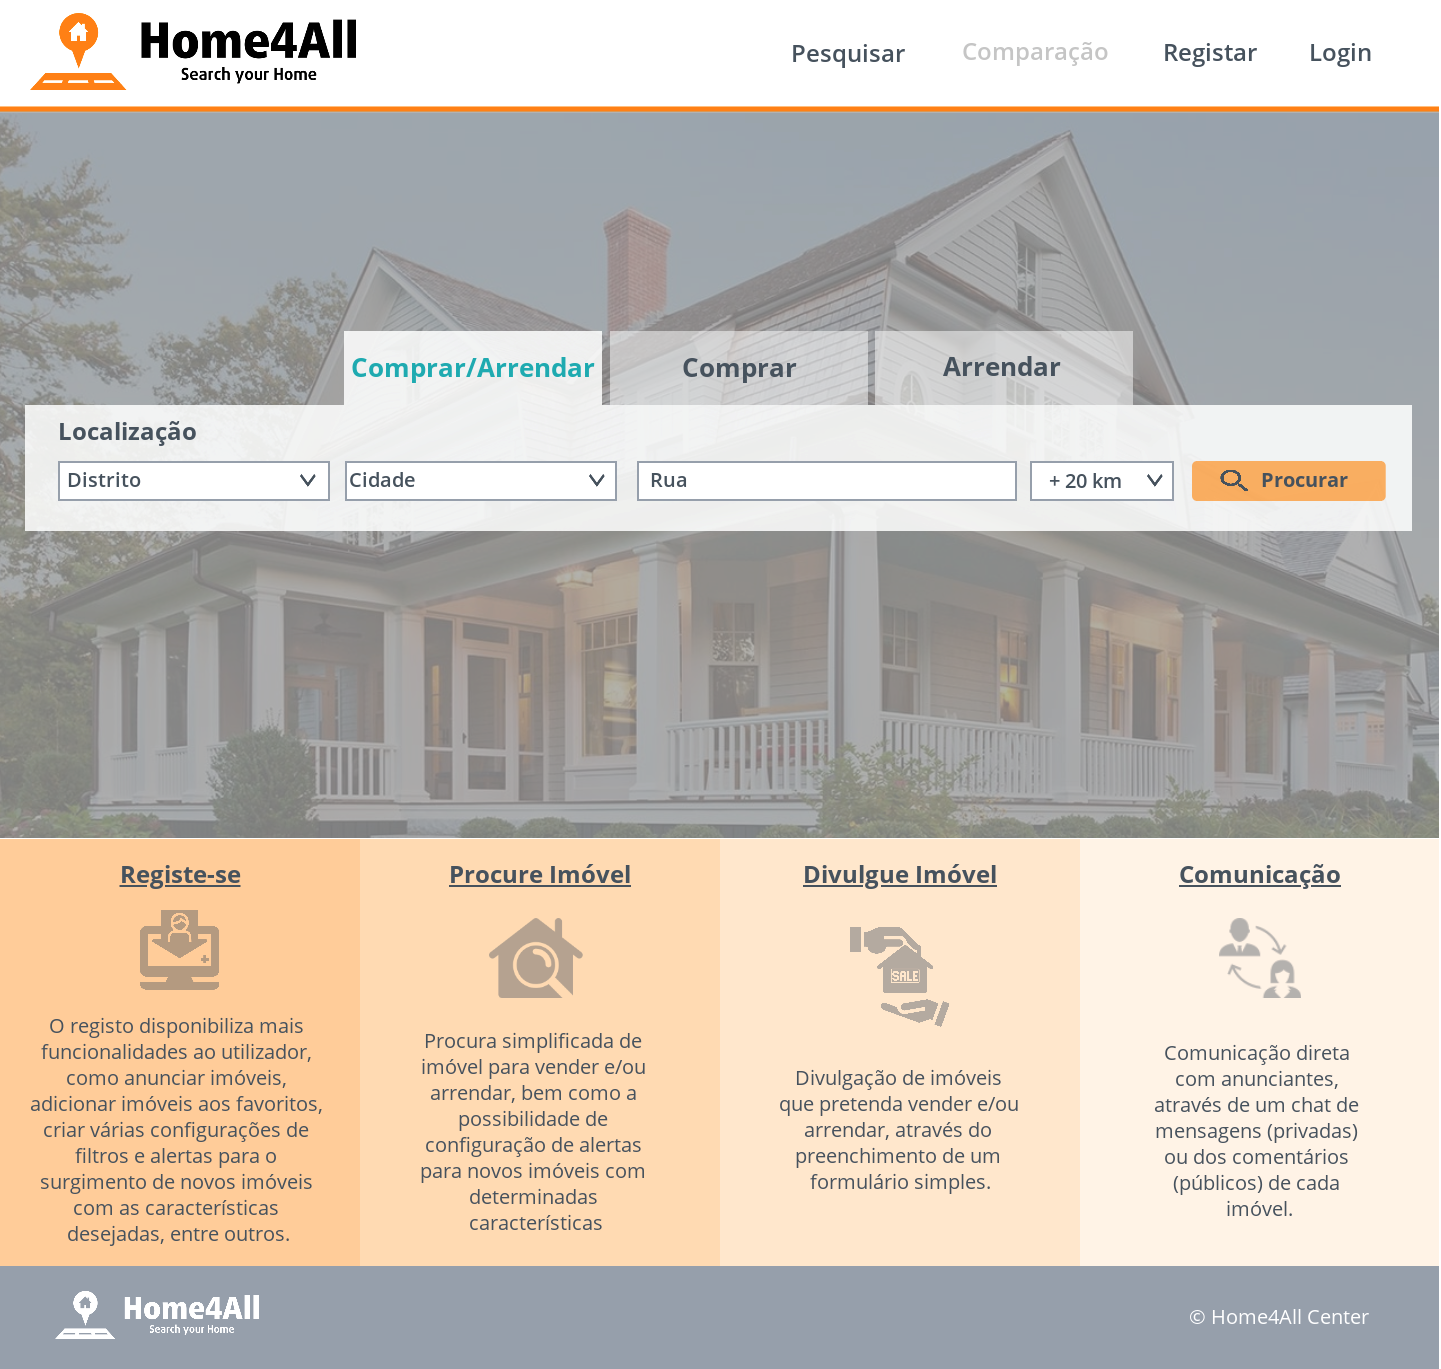
\includegraphics[width=0.9\textwidth]{./UI/Home_noLogin.png}
    \caption{\textit{Mockup} da página principal, sem \textit{login} efetuado.}
    \label{fig:home_no_login}
\end{figure}

Nesta página, salientam-se como princípios de usabilidade respeitados os que se apresentam de seguida:
\begin{itemize}
    \item \texttt{Learnability: Predictability} -- Inatividade do menu de ``Comparação'' permite ao utilizador prever que o sistema de comparação de imóveis não está disponível. Passando o rato sobre o menu surgirá a identificação do motivo (necessitam de ser adicionados pelo menos dois imóveis ao sistema de comparação).
    
    \item \texttt{Learnability: Familiarity} -- A cor do menu inativo (cinzento) é comummente utilizada para indicar que determinado botão ou elemento não está em funcionamento. Para além disso, o formato do menu principal e o sistema de pesquisa é semelhante aos de muitos outros \textit{websites}.
    
    \item \texttt{Learnability: Generalizability/Consistency} -- O menu principal é igual em todas as páginas, alterando apenas a formatação da funcionalidade selecionada e quais as funcionalidades disponíveis de acordo com o estado de autenticação (utilizador autenticado ou não autenticado).
    
    \item \texttt{Flexibility: Substitutivity} -- A distância pode ser escrita, como um inteiro (que é interpretado como estando em quilómetros), ou pode ser selecionada de entre as disponíveis.
    
    \item \texttt{Robustness: Observability} -- O utilizador pode perceber que não está autenticado pela presença das funcionalidades ``Registar'' e ``Login'' no menu principal. Para se autenticar, basta utilizar essas funcionalidades, que se encontram posicionadas de forma bem visível em qualquer página.
\end{itemize}

Relativamente aos padrões de \textit{design} utilizados, sobressaem-se os seguintes do \textit{website} \texttt{Designing Interfaces}:

\begin{itemize}
    \item \texttt{Clear Entry Points} -- A página principal do \textit{website} foca a atenção dos utilizadores nas caixas de texto onde se insere a localização para efetuar a pesquisa de imóveis. O menu principal e restante texto descritivo são vistos como elementos secundários.
    
    \item \texttt{Global Navigation} -- O menu principal aparece em todas as páginas do \textit{website} e apresenta um conjunto de ligações para as páginas mais importantes do mesmo.

    \item \texttt{Dropdown Chooser} -- O distrito, a cidade e a distância podem ser selecionados de um \textit{dropdown}, que contém uma coleção variada de valores que podem ser escolhidos.
    
    \item \texttt{Deep Background} -- A imagem de fundo, relacionada com o tema do \textit{website} (imóveis), foi introduzida para tornar a página principal mais atrativa e anunciar de forma evidente o tipo de produtos considerados no \textit{website}.
\end{itemize}

Por fim, dos \textit{design patterns} abordados no \textit{website} \texttt{Welie}, foram utilizados os seguintes:

\begin{itemize}
    \item \texttt{Home Link} -- O logótipo apresentado no canto superior esquerdo de todas as páginas do \textit{website} constitui uma ligação para a página principal.
    
    \item \texttt{Main Navigation} -- O menu principal é incluído em todas as páginas e está sempre visível, numa posição fixa.
    
    \item \texttt{Action Button} -- O botão ``Procurar'' permite ao utilizador realizar uma ação relevante no contexto da página atual, pelo que é realçado com recurso a um ícone, bem como a cor e formato distintos (retângulo laranja com cantos arredondados). Para além disso, o \textit{label} do botão incluí o verbo da ação.
    
    \item \texttt{Autocomplete} -- O campo da rua apresenta sugestões para completar o que está escrito, conforme o utilizador vai escrevendo.
\end{itemize}


\subsubsection{Pesquisa de Imóvel}

Relativamente à página de pesquisa de imóveis, optou-se por, para a localização, recorrer ao mesmo formato de pesquisa utilizado na página principal. Relativamente aos filtros e à ordenação dos resultados, apresenta-se os mesmos divididos por nome ou categoria, conforme se pode verificar no \textit{mockup} apresentado na figura \ref{fig:search}.

Para se adicionar um filtro ou alterar a ordenação dos resultados, tem de se clicar sobre a respetiva categoria e selecionar o filtro ou ordenação pretendido. O resultado de clicar sobre estas categorias é explicitado nos \textit{mockups} das figuras \ref{fig:search_filter01} a \ref{fig:search_ordination}.

A seleção de filtros ou alteração da ordenação implica a atualização automática dos resultados, caso a pesquisa por localização já tenha sido efetuada. Quando esta pesquisa é realizada, os resultados são apresentados conforme ilustrado no \textit{mockup} da figura \ref{fig:search_with_results}.

\begin{figure}[H]
    \centering
    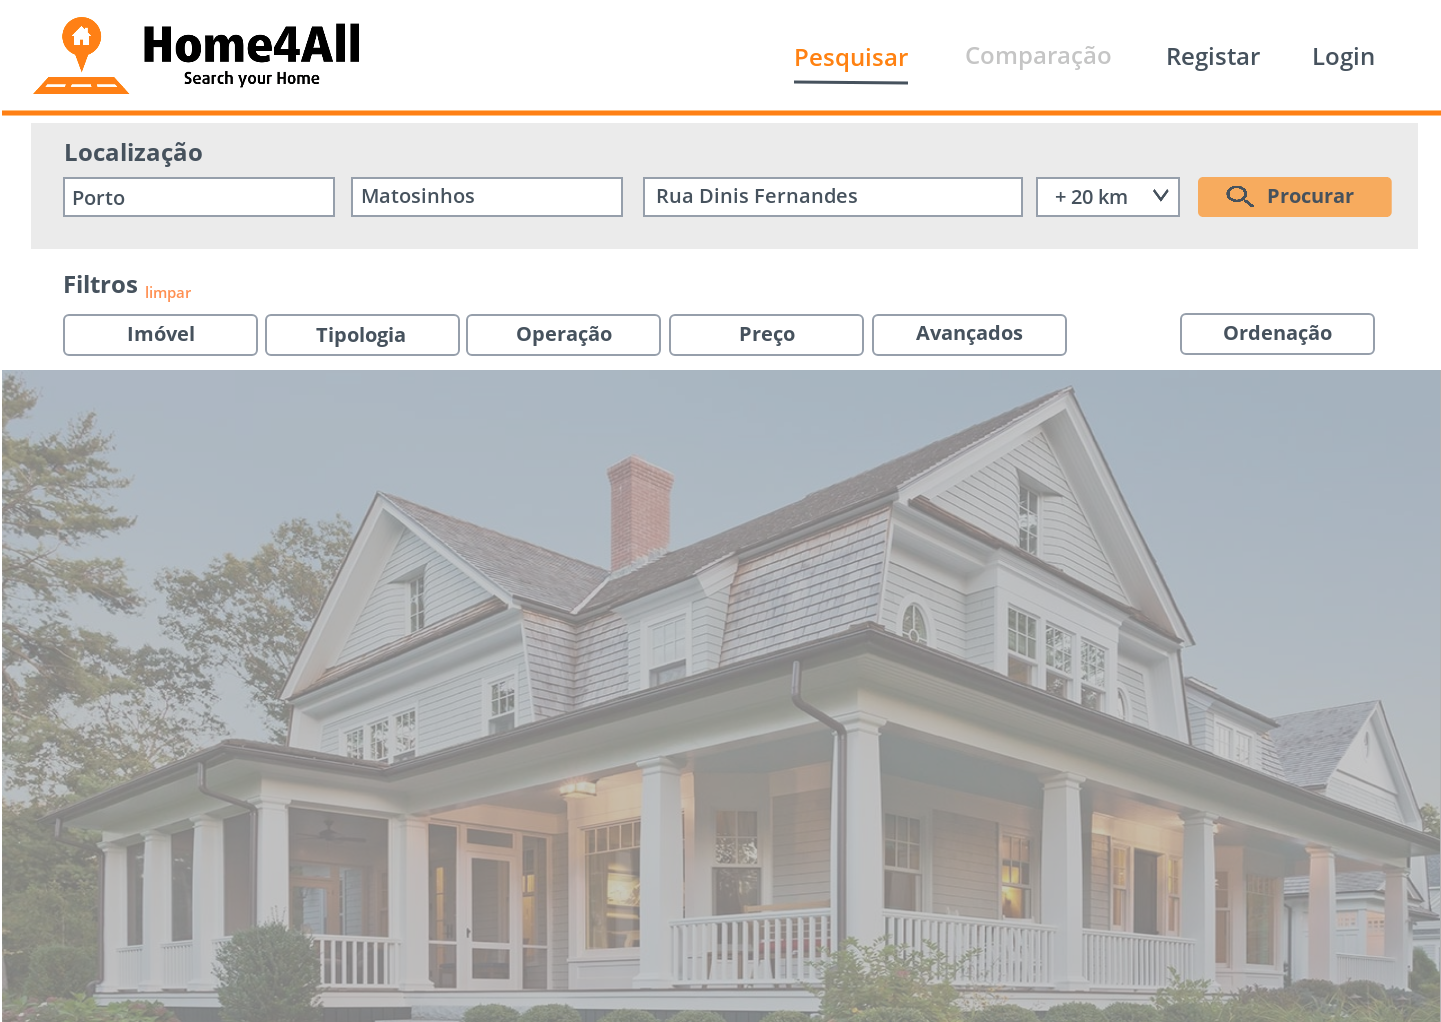
\includegraphics[width=0.9\textwidth]{./UI/Search.png}
    \caption{\textit{Mockup} da página de pesquisa, sem resultados nem \textit{login} efetuado.}
    \label{fig:search}
\end{figure}

\begin{figure}[H]
    \centering
    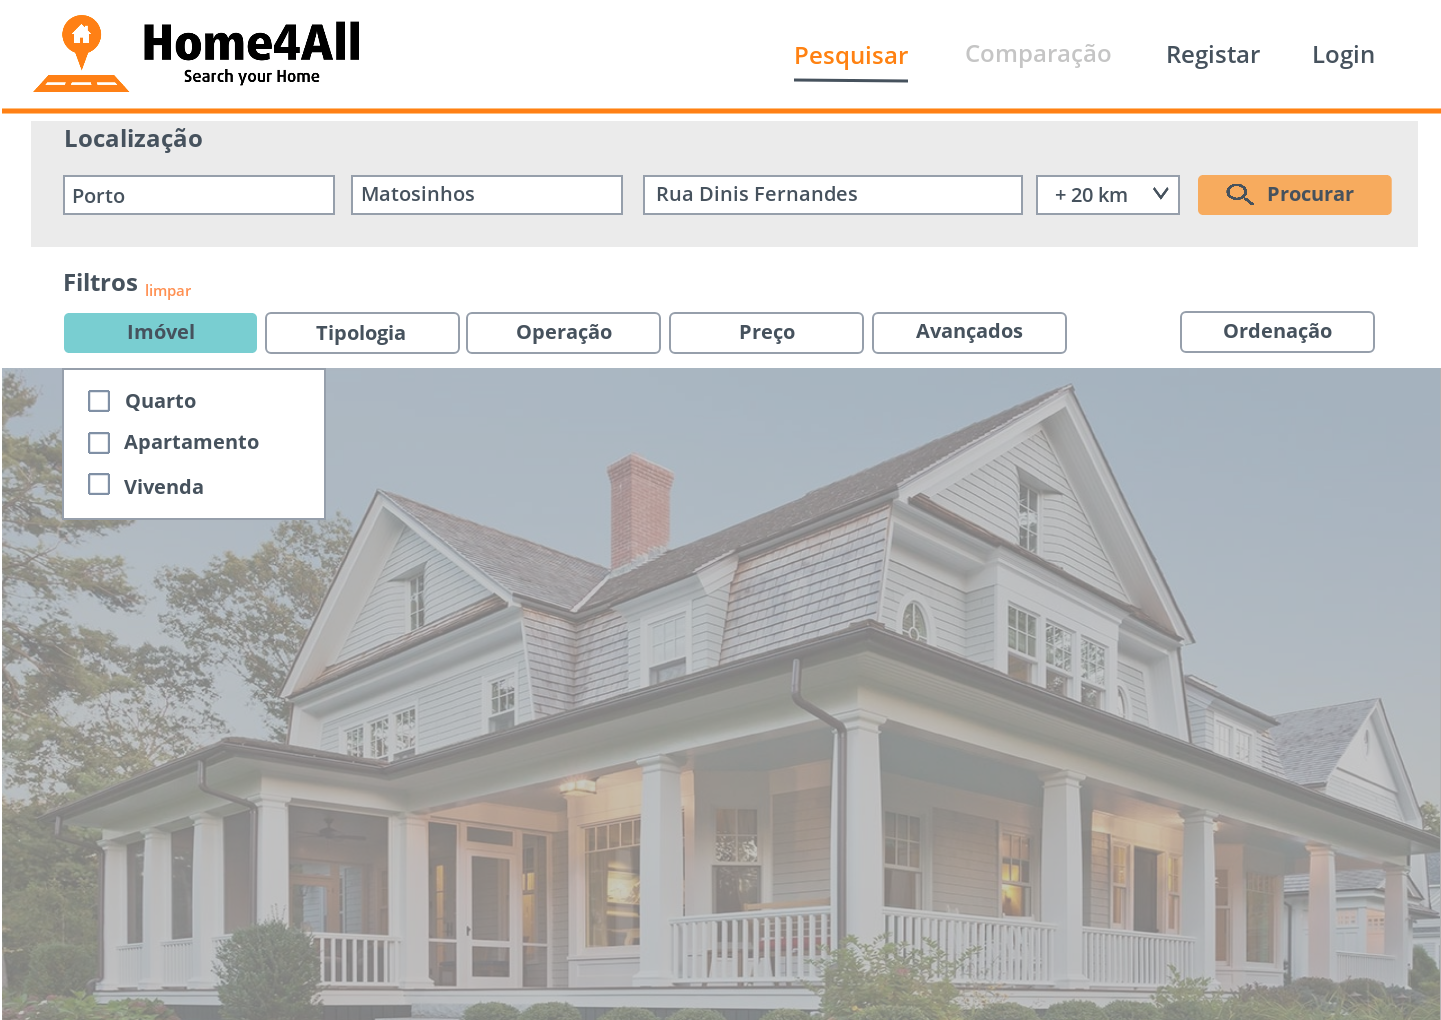
\includegraphics[width=0.9\textwidth]{./UI/Search_Filter01.png}
    \caption{\textit{Mockup} da página de pesquisa, com menu do filtro \texttt{Imóvel} aberto.}
    \label{fig:search_filter01}
\end{figure}

\begin{figure}[H]
    \centering
    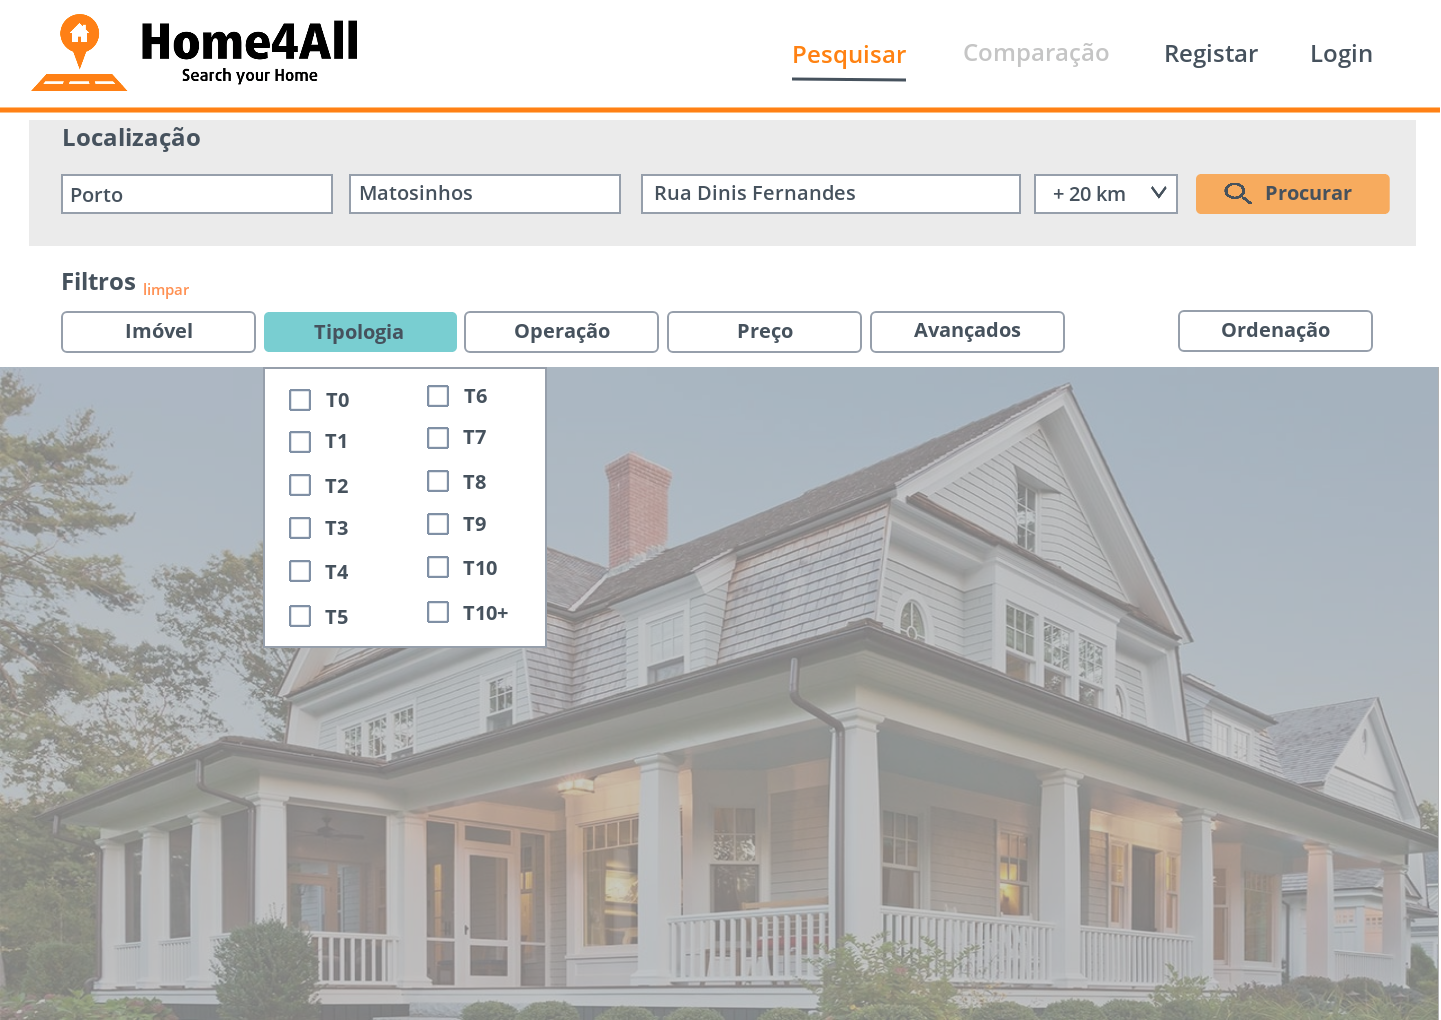
\includegraphics[width=0.9\textwidth]{./UI/Search_Filter02.png}
    \caption{\textit{Mockup} da página de pesquisa, com menu do filtro \texttt{Tipologia} aberto.}
    \label{fig:search_filter02}
\end{figure}

\begin{figure}[H]
    \centering
    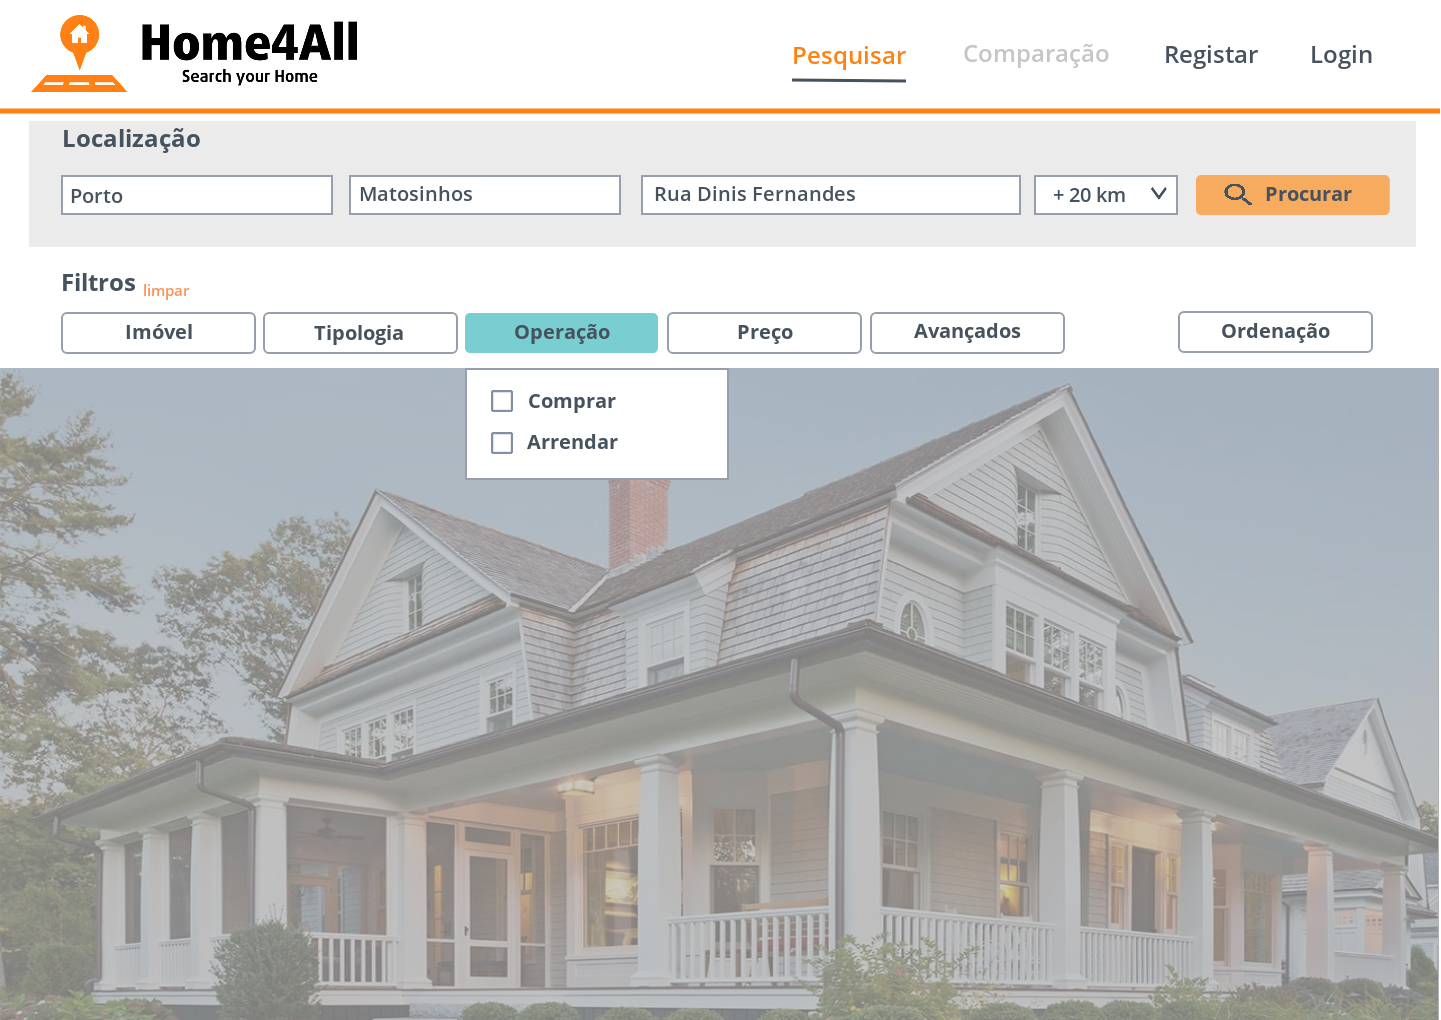
\includegraphics[width=0.9\textwidth]{./UI/Search_Filter03.png}
    \caption{\textit{Mockup} da página de pesquisa, com menu do filtro \texttt{Operação} aberto.}
    \label{fig:search_filter03}
\end{figure}

\begin{figure}[H]
    \centering
    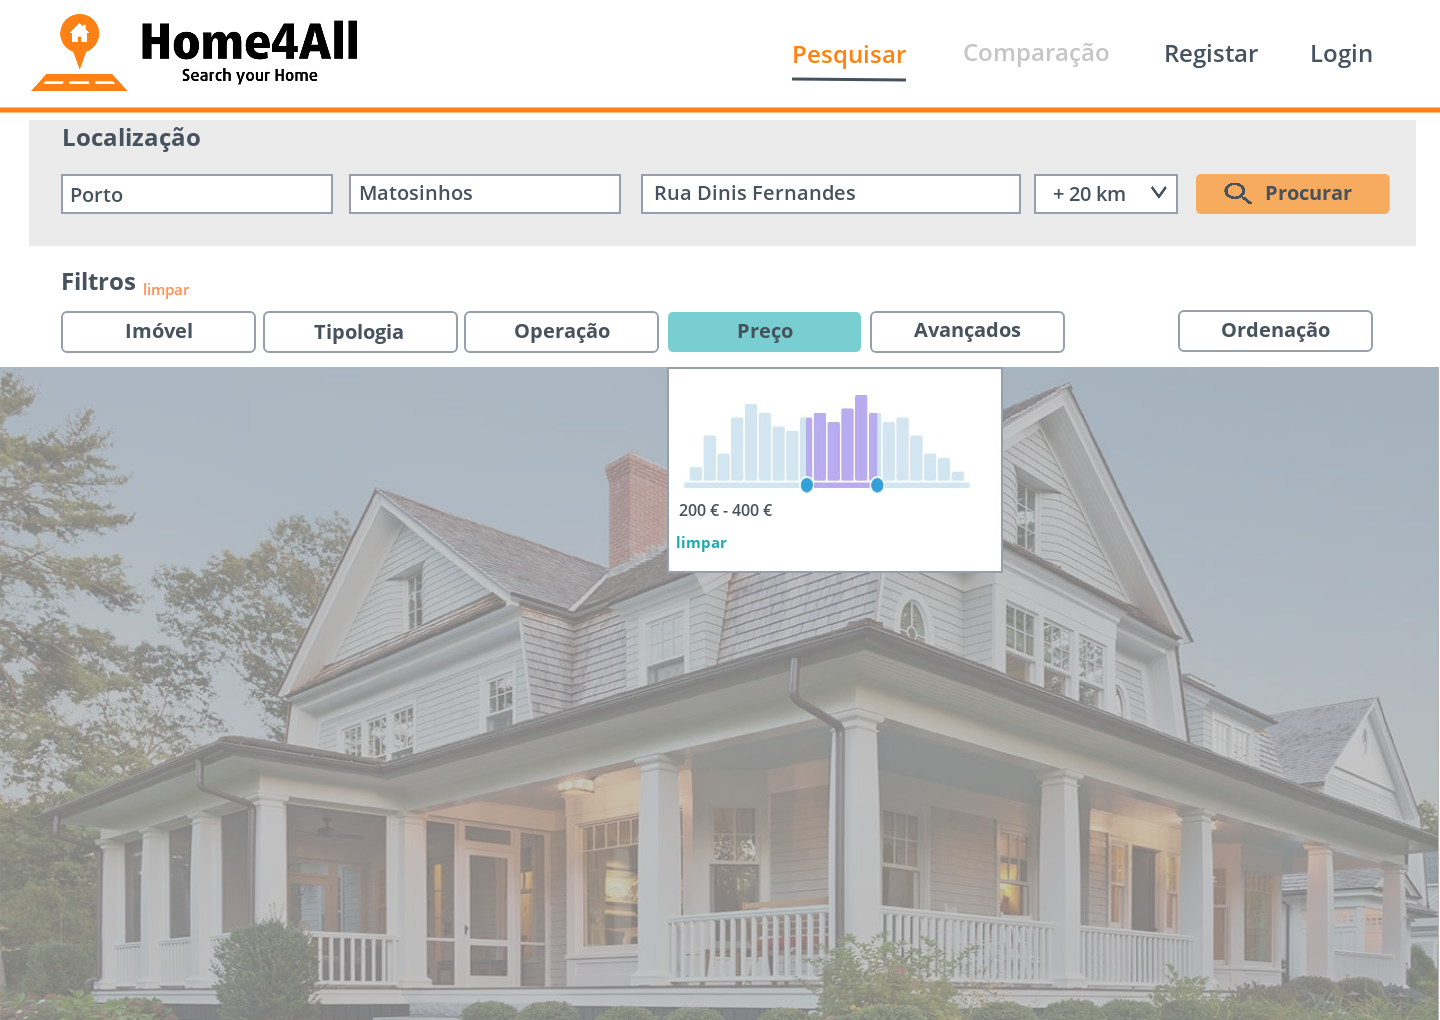
\includegraphics[width=0.9\textwidth]{./UI/Search_Filter04.png}
    \caption{\textit{Mockup} da página de pesquisa, com menu do filtro \texttt{Preço} aberto.}
    \label{fig:search_filter04}
\end{figure}

\begin{figure}[H]
    \centering
    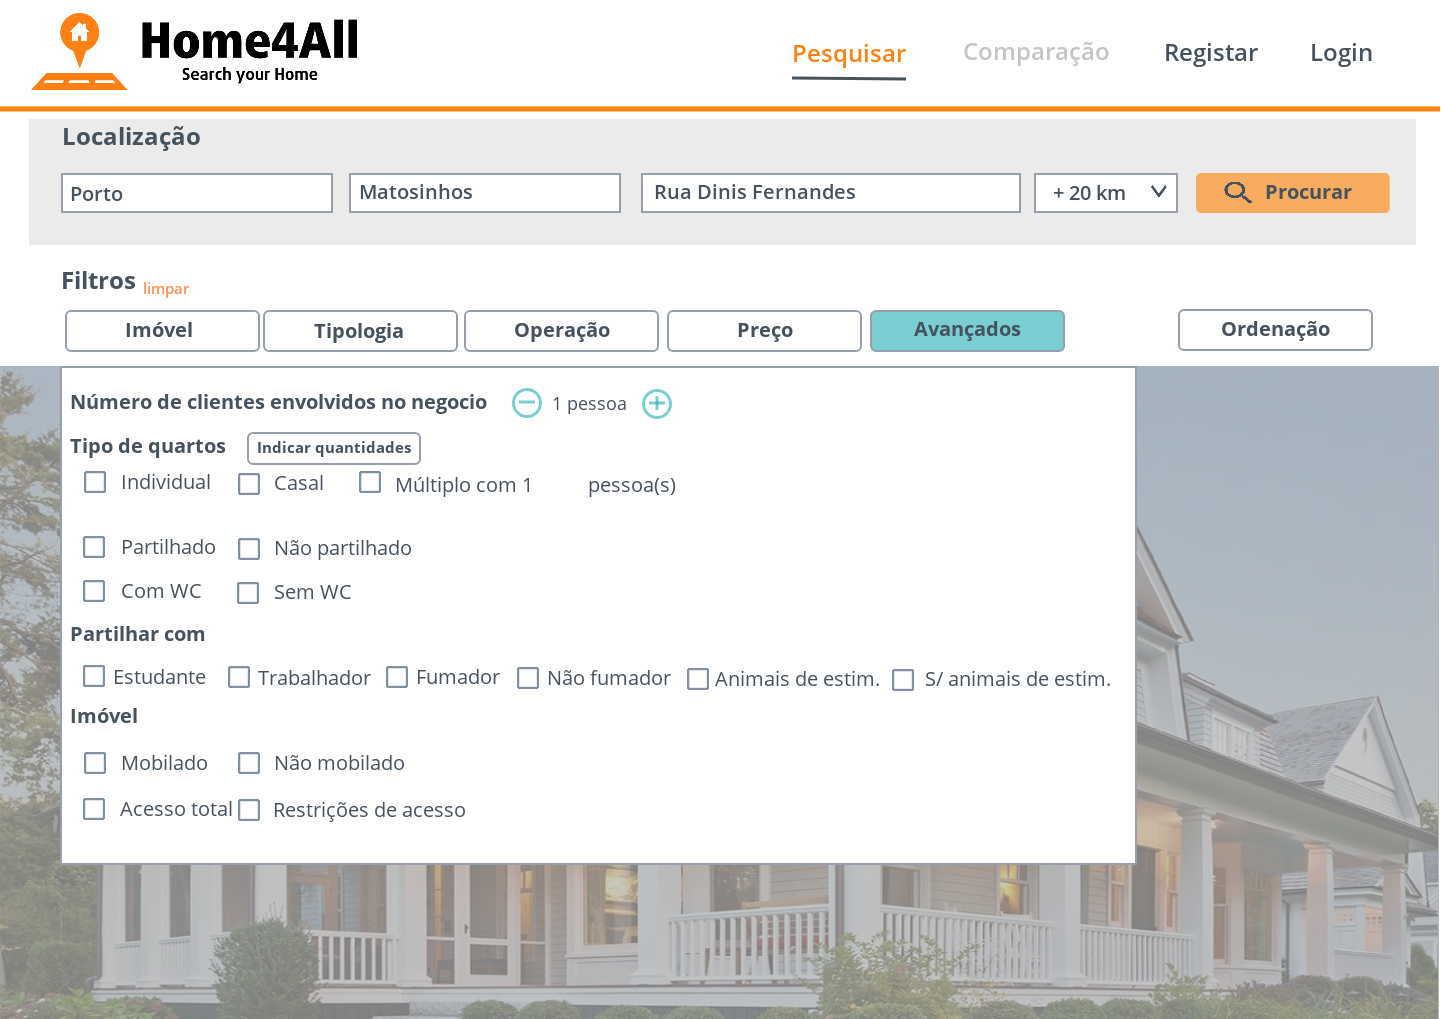
\includegraphics[width=0.9\textwidth]{./UI/Search_Filter05.png}
    \caption{\textit{Mockup} da página de pesquisa, com menu do filtro \texttt{Avançados} aberto.}
    \label{fig:search_filter05}
\end{figure}

\begin{figure}[H]
    \centering
    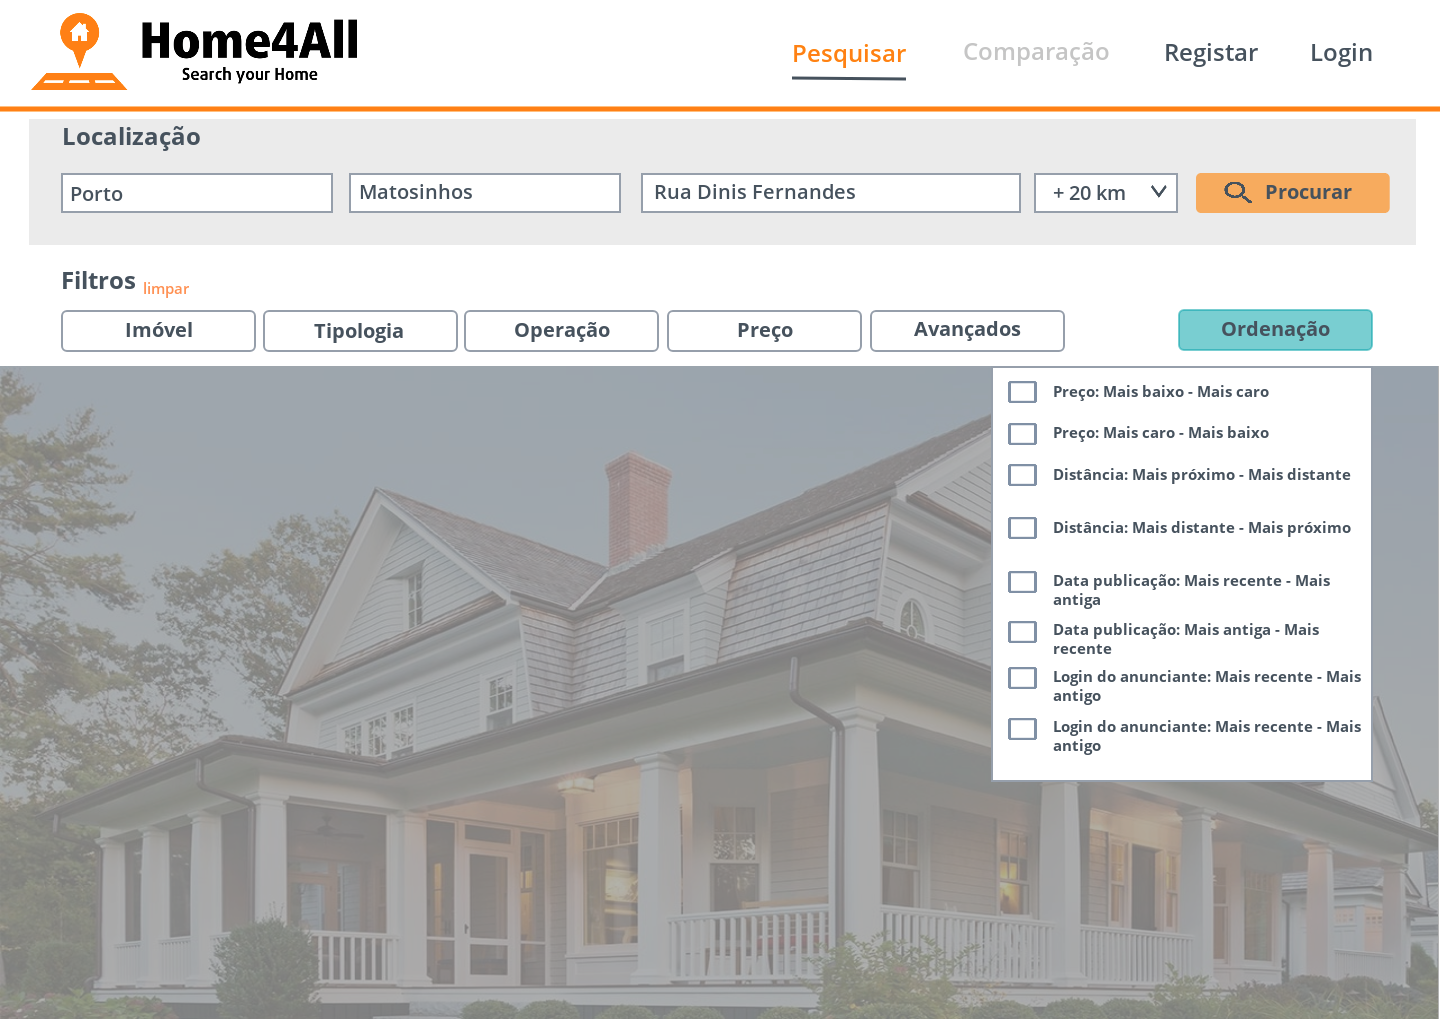
\includegraphics[width=0.9\textwidth]{./UI/Search_Ordination.png}
    \caption{\textit{Mockup} da página de pesquisa, com menu de \texttt{Ordenação} aberto.}
    \label{fig:search_ordination}
\end{figure}

\begin{figure}[H]
    \centering
    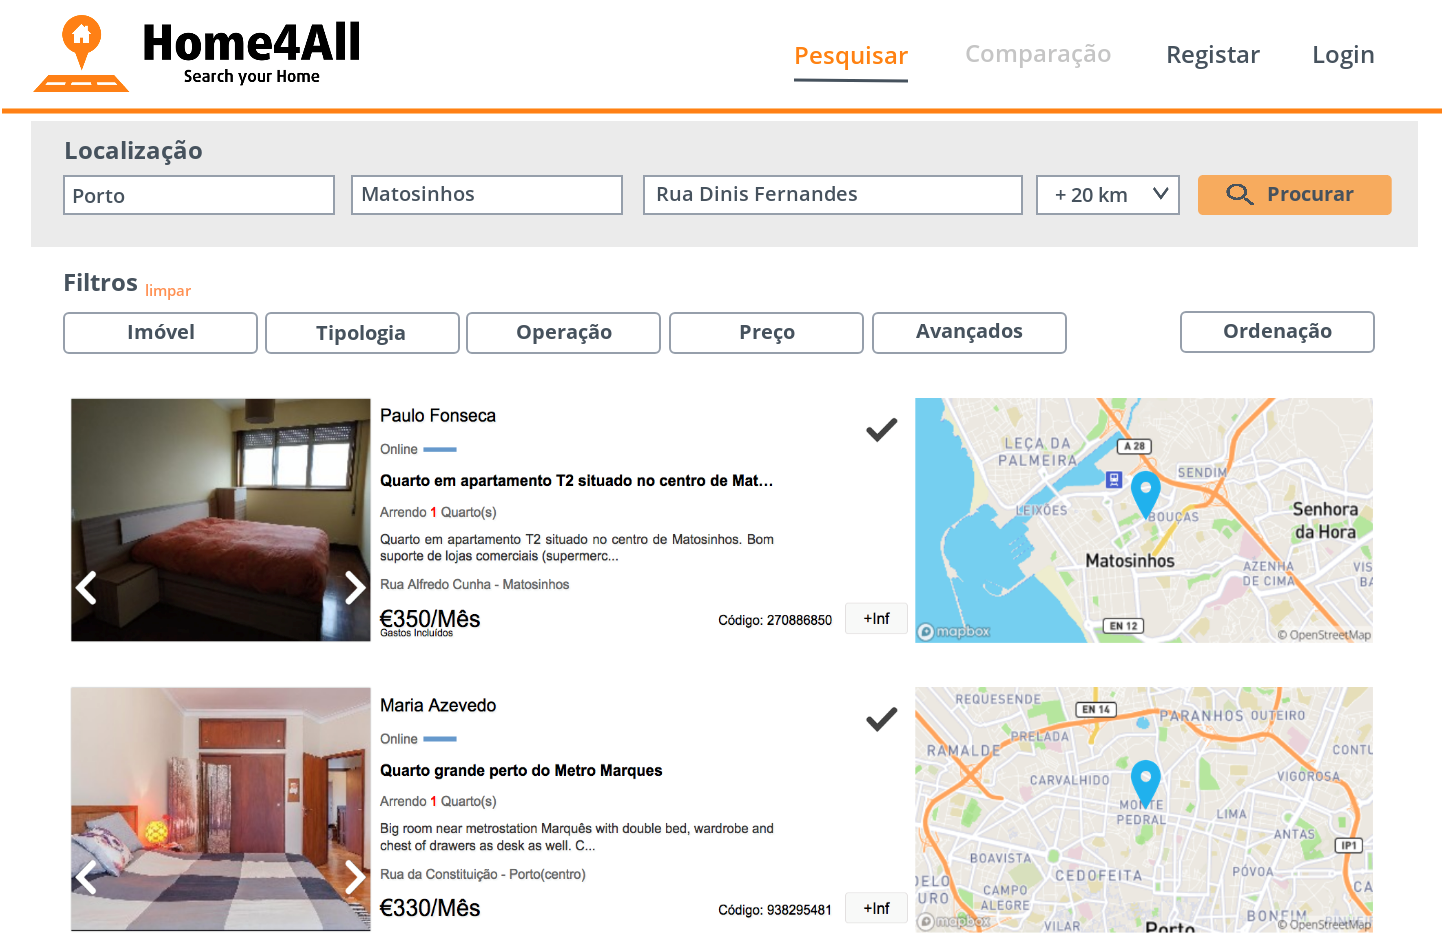
\includegraphics[width=0.9\textwidth]{./UI/Search_WithResults.png}
    \caption{\textit{Mockup} da página de pesquisa, com resultados.}
    \label{fig:search_with_results}
\end{figure}

Na pesquisa de imóveis, tiveram-se em principal consideração os seguintes princípios de usabilidade:

\begin{itemize}
    \item \texttt{Learnability: Predictability} -- Quando a seleção de determinado filtro tem como consequência o retorno de nenhum resultado, esse filtro aparece como desativado (cinzento).
    % DÚVIDA: Maior grau de previsibilidade se se indicar quantos serão selecionados por cada filtro

    \item \texttt{Learnability: Familiarity} -- O sistema de pesquisa e de filtros é semelhante ao de outros \textit{websites} de procura de qualquer tipo de produto, incluindo imóveis.
    
    \item \texttt{Learnability:  Generalizability/Consistency} -- Os filtros são selecionados sempre da mesma maneira e a área de pesquisa (localização) que aparece no topo da página é a mesma que a utilizada na página inicial (permitindo supor que o efeito no sistema será o mesmo).
    
    \item \texttt{Robustness: Observability} -- Os elementos necessários para efetuar uma (nova) pesquisa encontram-se bem visíveis para o utilizador. Para além disso, quando forem devolvidos muitos resultados, os imóveis serão apresentados de acordo com um sistema de paginação (\textit{browsability}).
\end{itemize}

Analisando os \textit{design patterns} disponibilizados pelo \textit{website} \texttt{Designing Interfaces}, conseguiu-se aplicar nesta página os apresentados de seguida:

\begin{itemize}
    \item \texttt{Dropdown Chooser} -- O distrito, a cidade e a distância podem ser selecionados de um \textit{dropdown}, que contém uma coleção variada de valores que podem ser escolhidos.
    
    \item \texttt{Deep Background} -- A imagem de fundo foi introduzida para preencher o espaço vazio aquando da inexistência de resultados e incentivar o utilizador a efetuar uma nova pesquisa para encontrar o seu imóvel ideal.
\end{itemize}

No \textit{website} \texttt{Welie} foi possível aplicar uma quantidade de padrões de \textit{design} superior, sendo estes os seguintes:

\begin{itemize}
    \item \texttt{Action Button} -- O botão ``Procurar'' permite ao utilizador realizar uma ação relevante no contexto da página atual, pelo que é realçado com recurso a um ícone, bem como a cor e formato distintos (retângulo laranja com cantos arredondados). Para além disso, o \textit{label} do botão incluí o verbo da ação.
    
    \item \texttt{Autocomplete} -- O campo da rua apresenta sugestões para completar o que está escrito, conforme o utilizador vai escrevendo.
    
    \item \texttt{Product Advisor} -- Os filtros que o utilizador pode selecionar permitem ao sistema aconselhá-lo sobre que imóveis deve consultar, tendo em conta restrições, preferências e necessidades do utilizador.
    
    \item \texttt{Map Navigator} -- A página de pesquisa com resultados utiliza este padrão para cada imóvel apresentado, de forma a facilitar a perceção do utilizador em relação à área onde o imóvel se localiza.
    
    \item \texttt{Paging} -- Conforme referido anteriormente, quando a quantidade de resultados apresentados for muito elevada, utilizar-se-á um sistema de \textit{paging}.
    
    \item \texttt{View} -- A página da pesquisa com resultados consiste numa vista geral sobre os vários imóveis disponíveis, tendo em conta as restrições indicadas. O utilizador pode consultar um imóvel clicando sobre o mesmo e depois retornar à lista de resultados, retrocedendo para a página anterior, selecionando a funcionalidade ``Pesquisa'' do menu principal ou clicando no botão ``Procurar'' (neste caso também pode alterar campos relativos à localização, podendo obter como resultado uma lista diferente).
\end{itemize}


\subsubsection{Consulta de imóvel}

Quanto à página de consulta de um imóvel, optou-se por inserir nesta toda a informação relativa ao imóvel, bem como a possibilidade de consultar a sua localização num mapa, enviar mensagem privada ao anunciante (se autenticado), adicionar o imóvel aos favoritos ou para comparação e consultar ou adicionar (se autenticado) comentários.

Procurou-se dispor a informação de forma simples e apelativa, para captar a atenção do cliente. Contudo, devido à elevada quantidade de informação, houve também uma grande preocupação em garantir uma disposição direta e facilmente percetível por parte do utilizador.

Ponderou-se ainda se a informação deveria ser dividida, por não caber toda no ecrã. Contudo, considerou-se que a apresentação da informação seguida é mais vantajosa, utilizando-se o \textit{scoll} para aceder aos dados não visíveis de forma imediata. Desta forma, o acesso à informação é mais rápido, não requerendo cliques de rato extra.
% DÚVIDA: Utilizar "Collapsible Panels" em dispositivos mais pequenos? 

Assim, o \textit{mockup} obtido para a página de consulta de um imóvel é apresentado na figura \ref{fig:property}.

\begin{figure}[H]
    \centering
    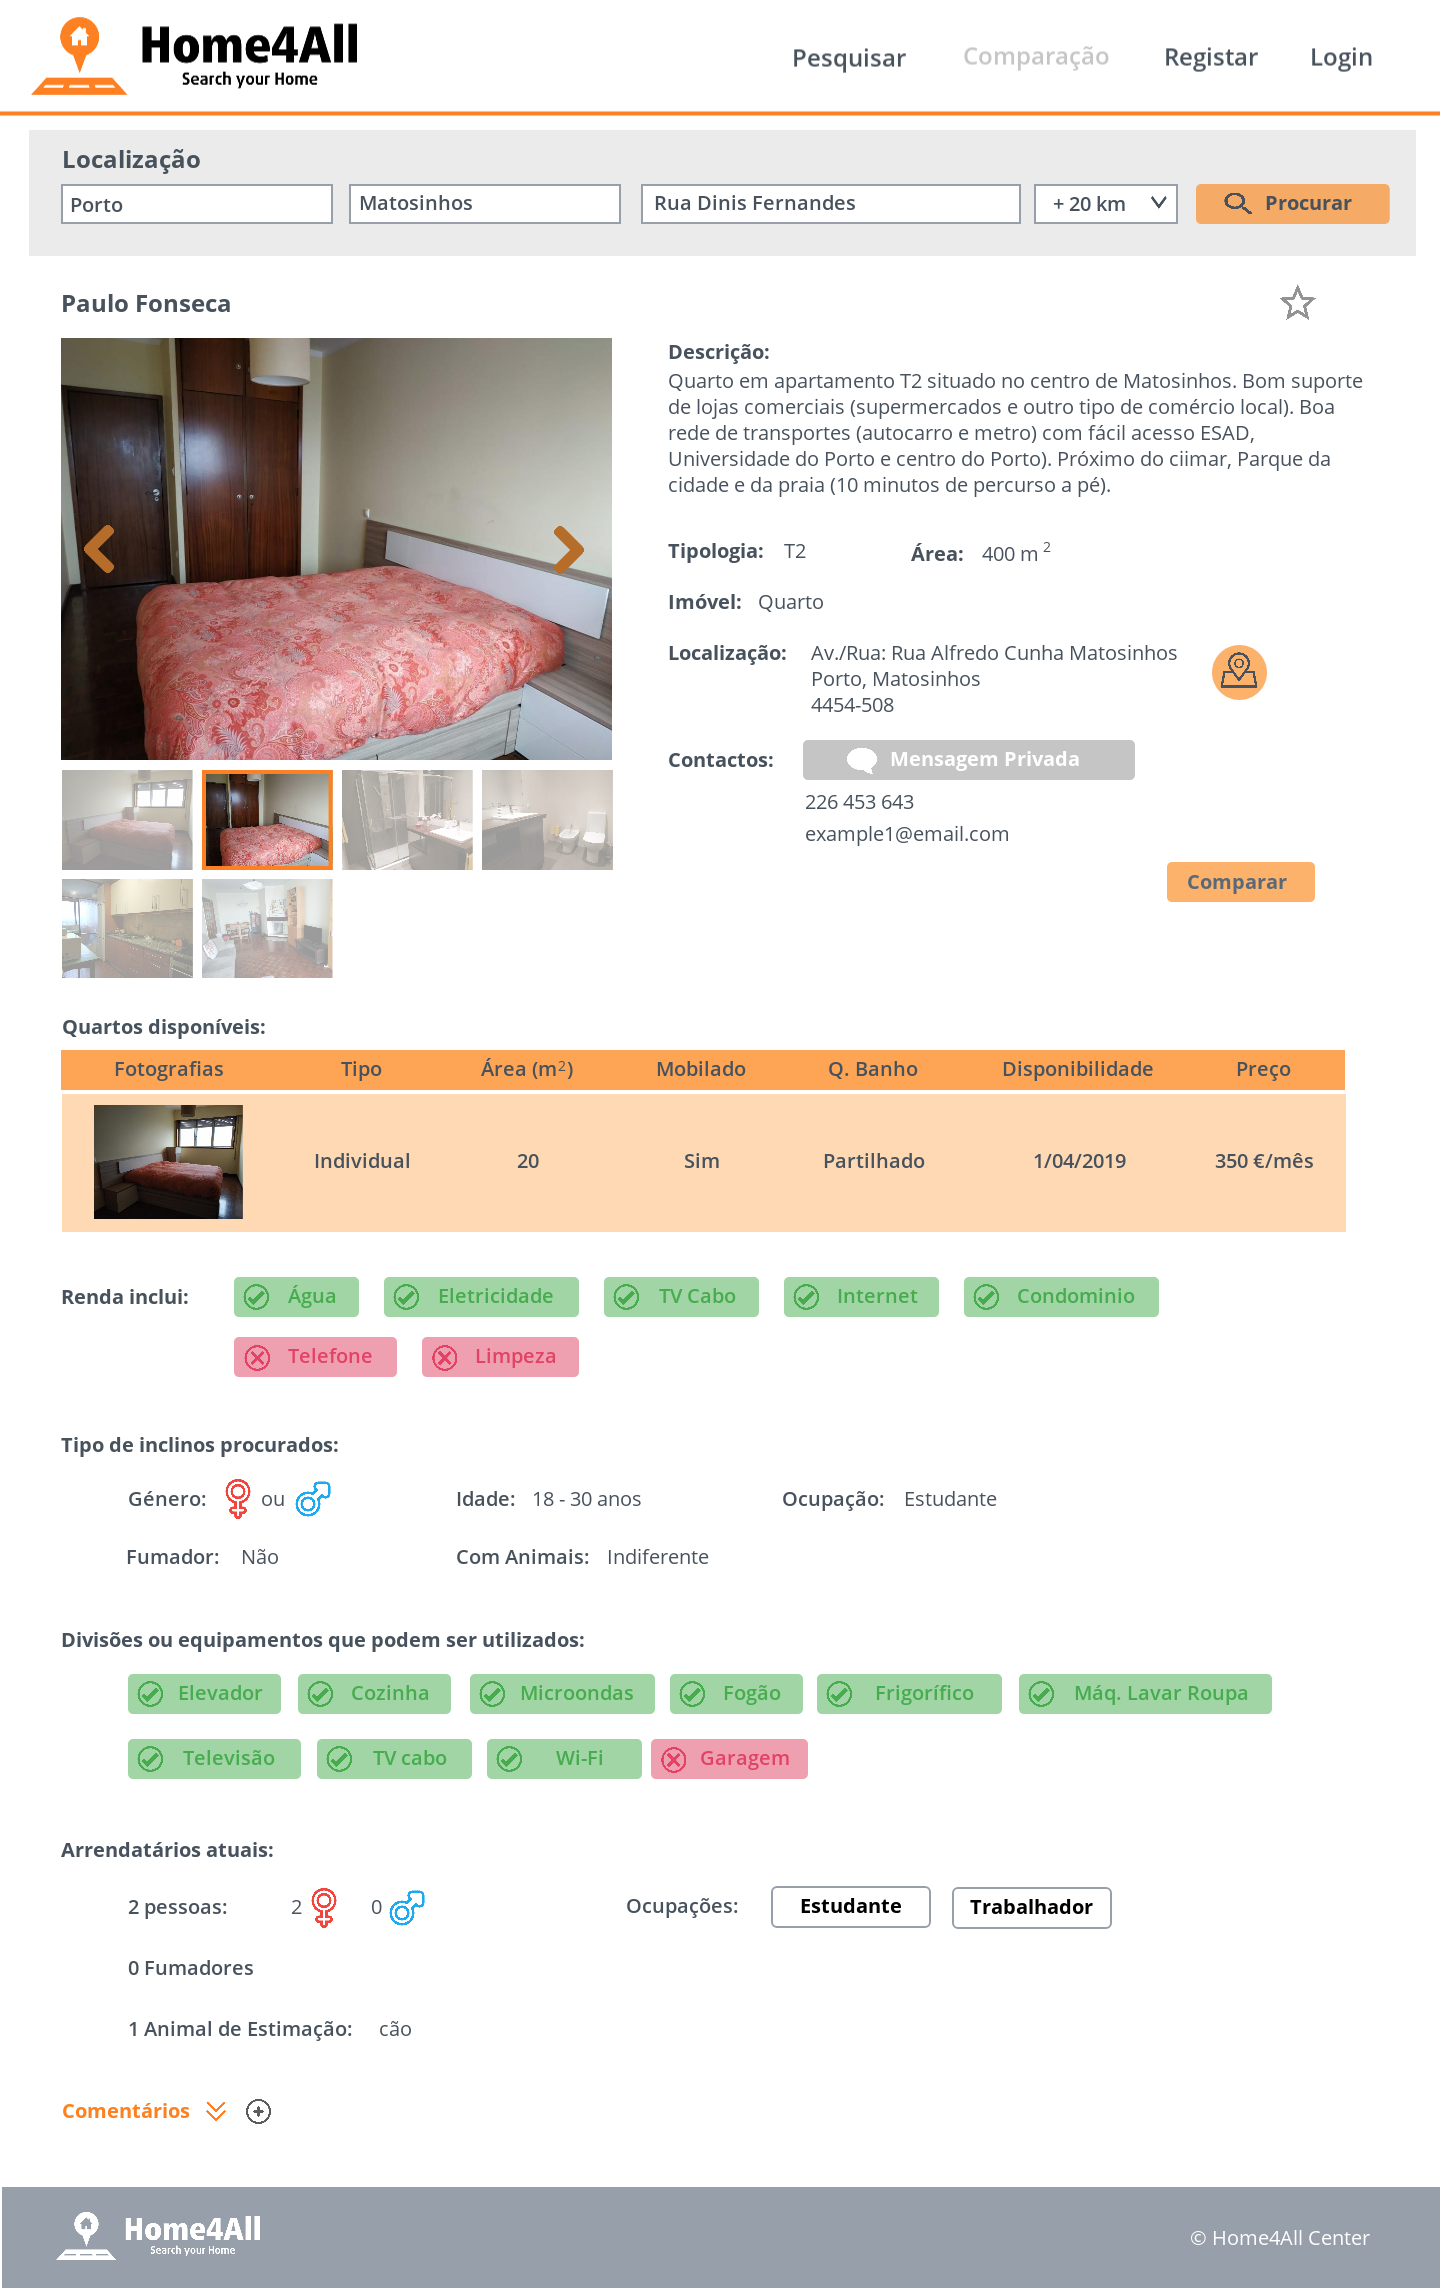
\includegraphics[width=0.85\textwidth]{./UI/Property.png}
    \caption{\textit{Mockup} da página com informações sobre um imóvel.}
    \label{fig:property}
\end{figure}

Nesta página consegue-se verificar os seguintes princípios de usabilidade:

\begin{itemize}
    \item \texttt{Learnability: Predictability} -- Inatividade dos botões de enviar mensagem privada ao anunciante e de adicionar imóvel aos favoritos permite ao utilizador prever que estas funcionalidades não estão disponíveis. Passando o rato sobre os botões surgirá a identificação do motivo (utilizador necessita de se autenticar primeiro).
    
    \item \texttt{Learnability: Synthesizability} -- Após adicionar ou remover o imóvel dos favoritos ou do sistema de comparação, surgirá na página uma mensagem efémera de sucesso ou insucesso. Para além disso, quando um imóvel já se encontra nos favoritos, o símbolo apresentado é de uma estrela completamente preenchida. Quando o imóvel não se encontra nos favoritos, apenas aparece o contorno da estrela. Para a comparação, se o imóvel ainda não está incluído, então o botão associado tem o \textit{label} ``Comparar''. Caso contrário, o \textit{label} é ``Não comparar''.
    
    \item \texttt{Learnability: Familiarity} -- A página de consulta do imóvel é semelhante a páginas de outros websites que descrevem qualquer tipo de produto, incluindo imóveis.
    
    \item \texttt{Learnability: Generalizability/Consistency}-- A existência do mesmo menu de pesquisa no topo da página permite supor que o efeito no sistema será o mesmo que quando aparecia na página de pesquisa e na página principal.
    
    \item \texttt{Robustness: Observability} -- Apesar das operações de consultar ou adicionar comentário não estarem imediatamente visíveis (ser necessário efetuar \textit{scroll}), considera-se que este fator não representará um impedimento para os clientes. De facto, muitos \textit{websites} também utilizam sistemas deste género, pelo que o utilizador já deverá estar acostumado.
\end{itemize}

Relativamente aos \textit{design patterns} do \textit{website} \texttt{Designing Interfaces}, apenas foi utilizado o \texttt{Extras On Demand}. Recorreu-se a este padrão para desenhar o surgimento do mapa com a localização do imóvel e a visualização dos comentários do imóvel. Como são informações adicionais sobre o imóvel (localização gráfica e questões públicas colocadas por outros clientes), considerou-se que estes dados apenas deveriam ser apresentados mediante solicitação por parte do utilizador.

Já do \textit{website} \texttt{Welie}, conseguiram-se utilizar mais padrões de \textit{design}:

\begin{itemize}
    \item \texttt{Map Navigator} -- Clicar no botão ao lado da ``Localização'' resulta no aparecimento de um mapa (no qual se pode navegar para outras localizações), com indicação da localização do respetivo imóvel.
    
    \item \texttt{Action Button} -- O botão ``Procurar'' permite ao utilizador realizar uma ação relevante no contexto da página atual, pelo que é realçado com recurso a um ícone, cor e formato distintos (retângulo laranja com cantos arredondados). Para além disso, o \textit{label} do botão inclui o verbo da ação.
    
    \item \texttt{Slideshow} -- As fotografias do imóvel são apresentadas cada uma por alguns segundos. Para além disso, é possível passar para a imagem seguinte/anterior, bem como selecionar uma imagem específica.
    
    \item \texttt{Collector} -- O imóvel pode ser adicionado a uma lista nos favoritos ou à lista dos imóveis no sistema de comparação, enquanto o utilizador o visualiza. A lista de imóveis para comparação está sempre acessível (se a lista tiver dois ou mais imóveis), enquanto que a dos favoritos necessita de autenticação, passando então a estar acessível a partir de qualquer página.
    
    \item \texttt{Thumbnail} -- Imagens dos imóveis mais pequenas são apresentadas para permitir ao utilizador consultar as fotografias que mais lhe interessar, de forma mais direta.
    
    \item \texttt{Comment Box} -- Ao clicar no botão de adicionar comentário, surge um pequeno formulário (com apenas um campo) para o utilizador autenticado inserir uma questão pública, a ser respondida pelo anunciante do imóvel.
\end{itemize}


\subsubsection{Comparação entre imóveis}

Para permitir uma comparação imediata entre as várias características dos imóveis selecionados, utilizou-se uma representação tabular da informação de cada imóvel, conforme solicitado nos requisitos. Essa representação pode ser consultada no \textit{mockup} apresentado na figura \ref{fig:property_comparison}.

\begin{figure}[H]
    \centering
    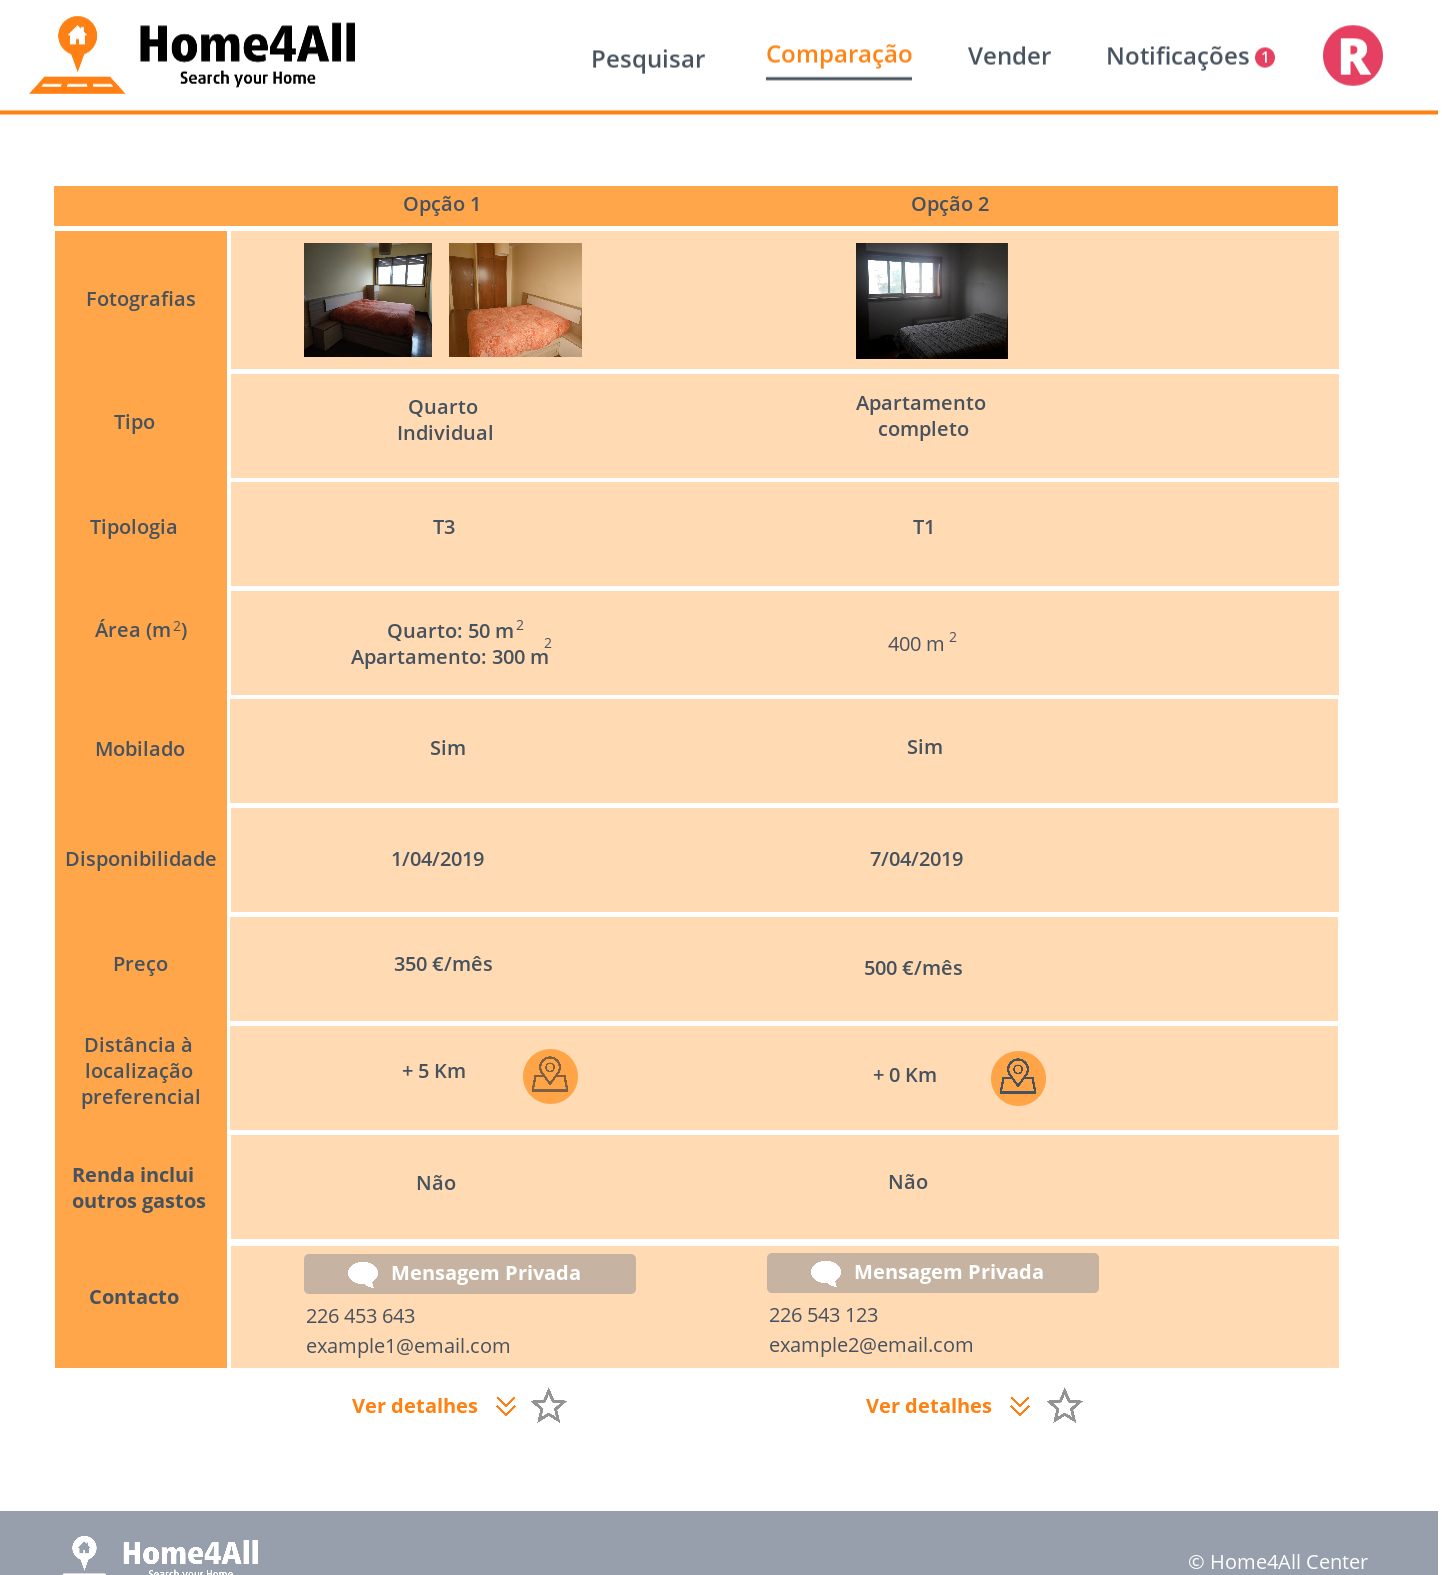
\includegraphics[width=0.9\textwidth]{./UI/PropertyComparison.png}
    \caption{\textit{Mockup} da página de comparação entre imóveis.}
    \label{fig:property_comparison}
\end{figure}

Em termos de princípios de usabilidade, salientam-se os seguintes:

\begin{itemize}
    \item \texttt{Learnability: Familiarity} -- Sistemas de comparação baseados em tabela são bem conhecidos e percetíveis por parte de qualquer tipo de utilizador.
    
    \item \texttt{Learnability: Generalizability/Consistency} -- As funcionalidades de visualização do imóvel no mapa, envio de mensagem privada ao anunciante e adição do imóvel aos favoritos são executadas da mesma forma (com o mesmo tipo de elementos) que na página de consulta do imóvel.
    
    \item \texttt{Robustness: Observability} -- As operações de adicionar aos favoritos e consultar imóvel não estão imediatamente visíveis, isto é, é necessário fazer \textit{scroll} para as visualizar. Contudo, estas não são as principais tarefas a executar nesta página, ao contrário da análise de comparação. Após essa análise é que faz sentido considerar realizar uma das outras ações.
\end{itemize}

Mais uma vez, dos \textit{design patterns} do \textit{website} \texttt{Designing Interfaces} apenas se utilizou o \texttt{Extras On Demand}. Recorreu-se a este padrão para desenhar o surgimento do mapa com a localização do imóvel e a visualização dos detalhes de um dos imóveis.

Relativamente ao \textit{website} \texttt{Welie}, conseguiram-se utilizar os seguintes padrões de \textit{design}:

\begin{itemize}
    \item \texttt{Map Navigator} -- Clicar no botão incluído na área da localização resulta no aparecimento de um mapa (no qual se pode navegar para outras localizações), com indicação da localização do respetivo imóvel.
        
    \item \texttt{Thumbnail} -- Imagens dos imóveis mais pequenas são apresentadas para permitir ao utilizador ter uma visão geral das várias fotografias e consultar as que mais lhe interessar, de forma direta.
    
    \item \texttt{Product Comparison} -- É apresentada uma matriz de imóveis e características dos mesmos, para facilitar ao utilizador a comparação entre eles.
\end{itemize}


\subsubsection{Registo}

A página de registo foi desenhada com um formato \textit{standard}, permitindo o recurso a contas do Facebook ou da Google. Caso seja utilizada uma conta externa no registo, serão posteriormente solicitados ao utilizador dados de contacto, idade, género e profissão.

O \textit{mockup} desta página é apresentado na figura \ref{fig:register}.

\begin{figure}[H]
    \centering
    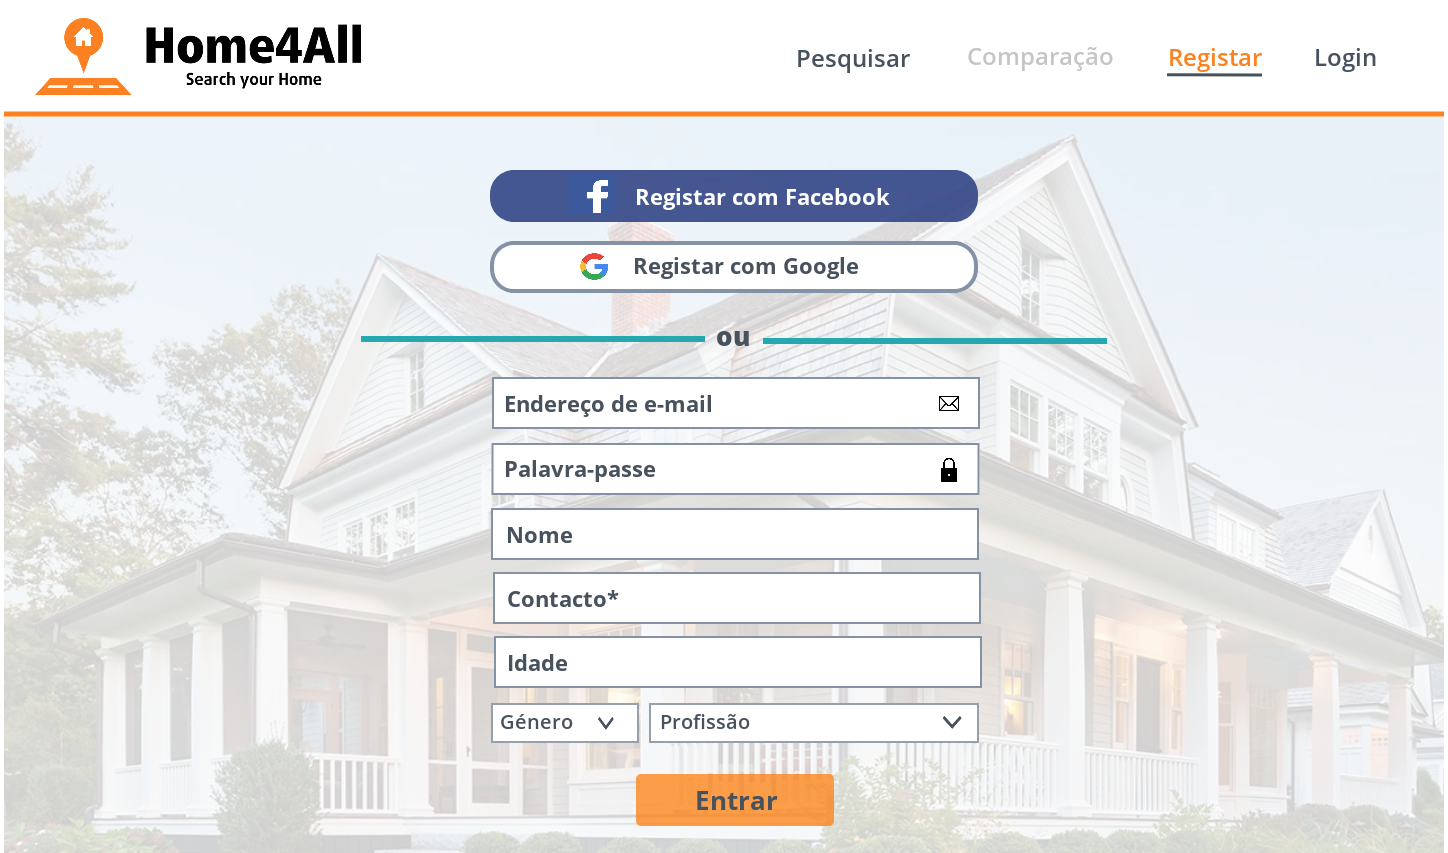
\includegraphics[width=0.9\textwidth]{./UI/Register.png}
    \caption{\textit{Mockup} da página de registo.}
    \label{fig:register}
\end{figure}

Relativamente aos princípios de usabilidade aplicáveis a esta página, destacam-se os seguintes:

\begin{itemize}
    \item \texttt{Learnability: Synthesizability} -- Após clicar no botão ``Entrar'' (registo), será indicada uma mensagem de sucesso ou insucesso. No primeiro caso, será ainda efetuada automaticamente a autenticação do utilizador. No segundo caso, será indicado o motivo do insucesso.
    
    \item \texttt{Learnability: Familiarity} -- O sistema de registo é semelhante ao de outros \textit{websites}.
    
    \item \texttt{Flexibility: Substitutivity} -- O contacto pode ser escrito com ou sem o respetivo indicativo de país.
    
    \item \texttt{Robustness: Observability} -- O botão para registo está visível em ecrãs médios e grandes. No caso de ecrãs pequenos, o botão aparece imediatamente a seguir ao respetivo formulário, de preenchimento obrigatório.
\end{itemize}


Entre os padrões de \textit{design} do \textit{website} \texttt{Designing Interfaces}, utilizou-se o \texttt{Dropdown Chooser} para se indicar um género ou profissão, tendo em conta as disponíveis. 

Quanto ao \textit{website} \texttt{Welie}, utilizaram-se os seguintes \textit{design patterns}:

\begin{itemize}
    \item \texttt{Action Button} -- O botão ``Entrar'' permite ao utilizador realizar a ação principal no contexto da página atual, pelo que é realçado com recurso a uma cor e um formato distintos (retângulo laranja com cantos arredondados). Para além disso, o \textit{label} do botão inclui o verbo da ação.

    \item \texttt{Registration} -- A página de registo fornece ao utilizador a possibilidade de armazenar os seus dados pessoais, para posterior utilização.
\end{itemize}


\subsubsection{\textit{Login}}

A página de \textit{login} também foi desenhada com um formato \textit{standard} e semelhante à do registo, permitindo a autenticação com uma conta Facebook ou Google. O \textit{mockup} desta página é apresentado na figura \ref{fig:login}.

\begin{figure}[H]
    \centering
    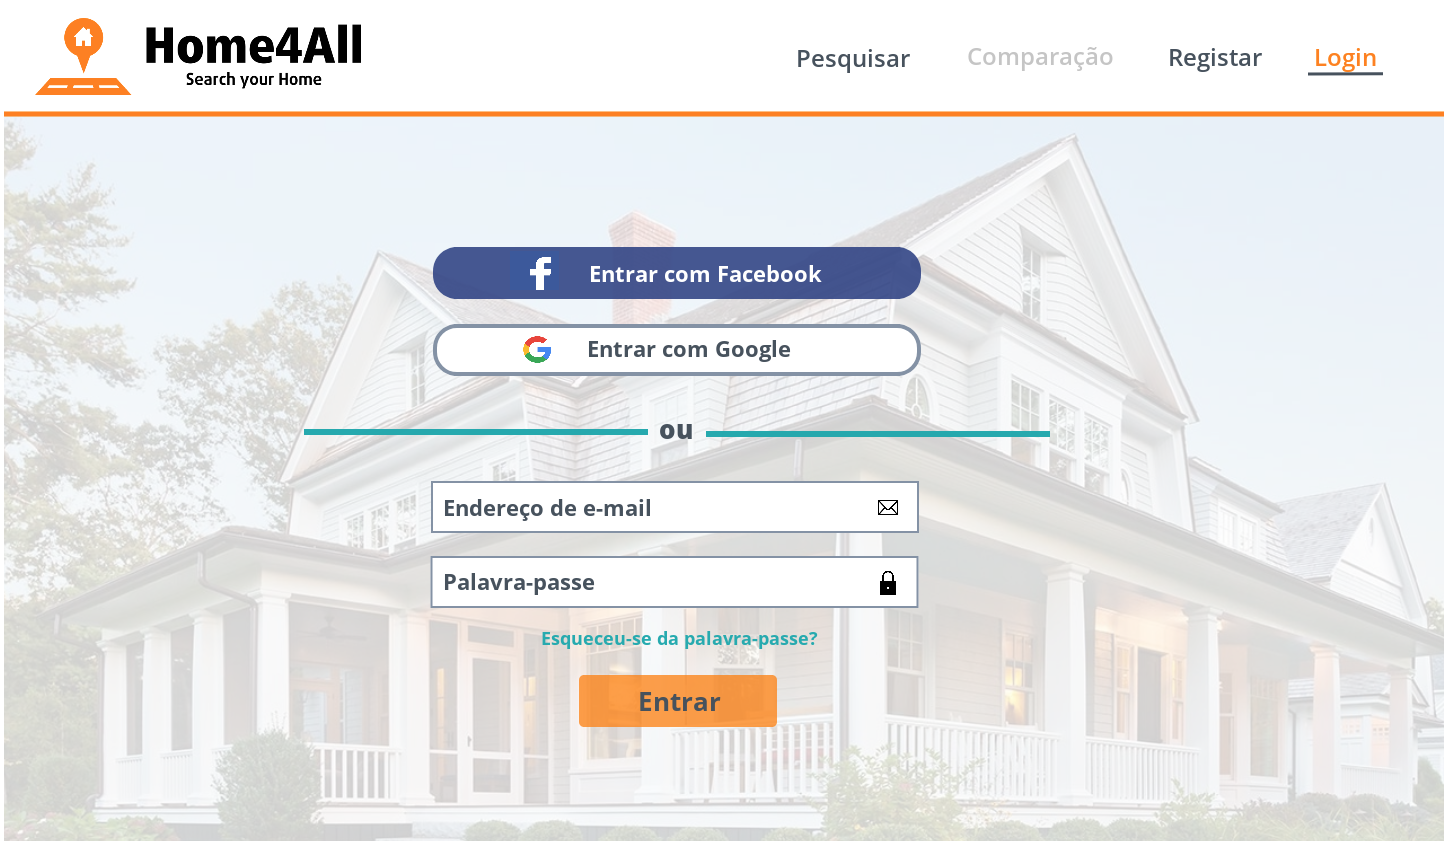
\includegraphics[width=0.9\textwidth]{./UI/Login.png}
    \caption{\textit{Mockup} da página de \textit{login}.}
    \label{fig:login}
\end{figure}


Nesta página sobressai-se a aplicação dos seguintes princípios de usabilidade:

\begin{itemize}
    \item \texttt{Learnability: Synthesizability} -- Após clicar no botão ``Entrar'' (\textit{login}), será indicada uma mensagem de sucesso ou insucesso. No primeiro caso, será de seguida apresentada a página com os dados pessoais do utilizador.
    
    \item \texttt{Learnability: Familiarity} -- O sistema de \textit{login} é semelhante ao de outros \textit{websites}.
    
    \item \texttt{Flexibility: Generalizability/Consistency} -- Os campos de \textit{login} têm a mesma formatação que os respetivos campos de registo. Salienta-se que o botão de submissão do formulário destas páginas é igual, devido ao estado do sistema passar a ser o mesmo nos dois casos (utilizador autenticado), caso a respetiva ação seja efetuada com sucesso.
    
    \item \texttt{Robustness: Observability} --  O botão de \textit{login} está visível em ecrãs médios e grandes. No caso de ecrãs pequenos, o botão aparece imediatamente a seguir ao respetivo formulário, de preenchimento obrigatório.
\end{itemize}

Relativamente aos padrões de \textit{design} do \textit{website} \texttt{Designing Interfaces}, não se encontrou nenhum que fosse útil aplicar nesta página.

Quanto ao \textit{website} \texttt{Welie}, optou-se por utilizar os seguintes \textit{design patterns}:

\begin{itemize}
    \item \texttt{Action Button} -- O botão ``Entrar'' permite ao utilizador realizar a ação principal no contexto da página atual, pelo que é realçado com recurso a uma cor e um formato distintos (retângulo laranja com cantos arredondados). Para além disso, o \textit{label} do botão inclui o verbo da ação.

    \item \texttt{Login} -- A página de \textit{login} permite que o sistema identifique o respetivo utilizador, de forma a possibilitar o recurso a mais funcionalidades e a realização de pesquisas mais personalizadas.
\end{itemize}


\subsubsection{Página Principal (com \textit{login})}

Após a autenticação, as páginas de pesquisa e comparação previamente apresentadas continuam acessíveis, alterando apenas ligeiramente o menu principal. Através deste, passam a ser acessíveis as seguintes páginas:
% TODO:
\begin{itemize}
    \item ``Meus Anúncios'' -- permite a consulta, alteração, adição e remoção de anúncios efetuados pelo utilizador autenticado;
    \item ``Notificações'' --  permite o acesso direto à página de novos imóveis que cumpram as configurações especificadas;
    \item ``Dados do Perfil'' -- permite a consulta e alteração de dados diretamente relacionados com o perfil do utilizador autenticado;
    \item ``Configurações'' -- permite a consulta, alteração, adição e remoção de configurações de notificação;
    \item ``Favoritos'' -- permite a consulta de páginas marcadas pelo utilizador autenticado e reorganização da estrutura de armazenamento das mesmas.
\end{itemize}

A página principal do \textit{website}, agora com autenticação, é apresentada no \textit{mockup} da figura \ref{fig:home_with_login}.

\begin{figure}[H]
    \centering
    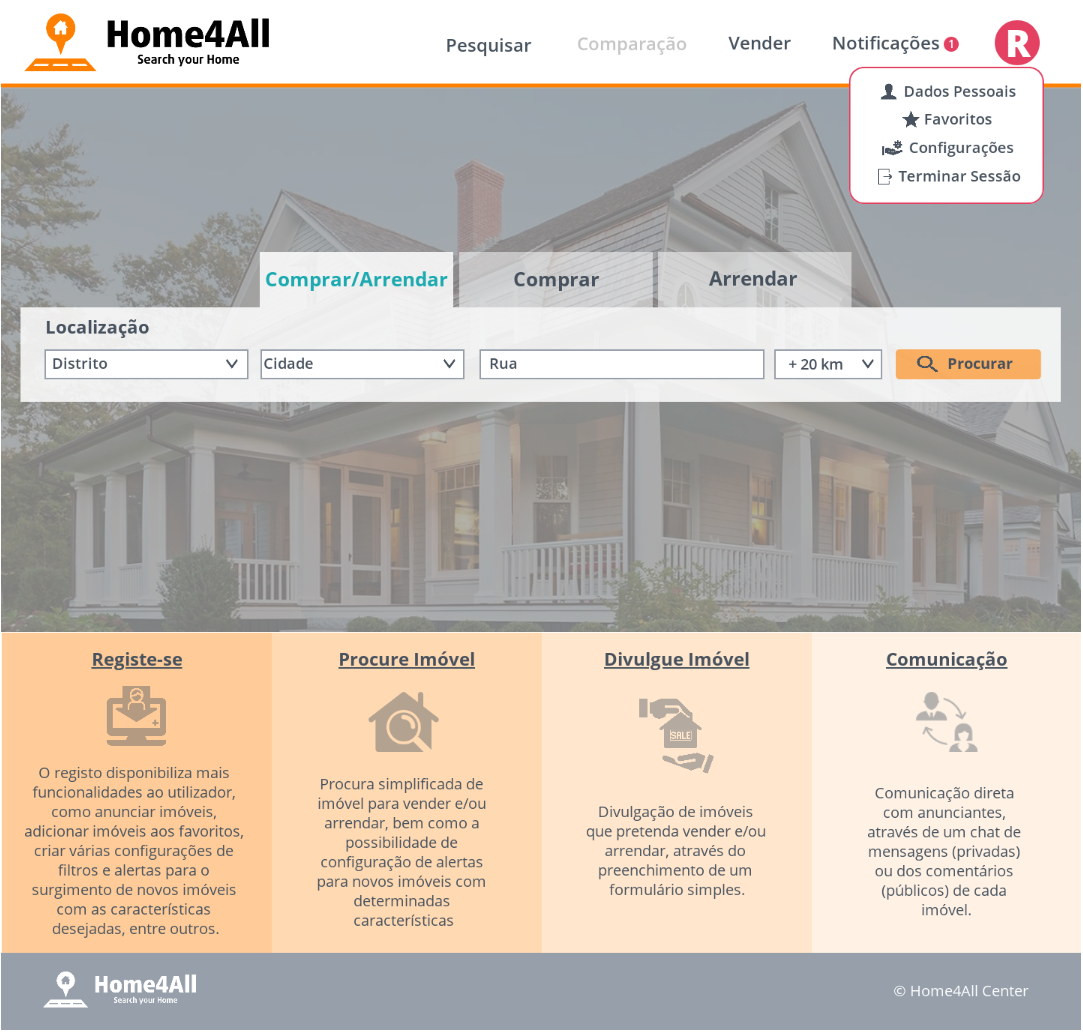
\includegraphics[width=0.9\textwidth]{./UI/Home_Login_Menu.png}
    \caption{\textit{Mockup} da página principal, com \textit{login} efetuado.}
    \label{fig:home_with_login}
\end{figure}

Esta página principal é igual à previamente apresentada, tendo apenas alterações no conteúdo do menu principal. Assim, ainda se aplicam os mesmos princípios e padrões de \textit{design} apresentados na secção \ref{fig:home_no_login}.

Contudo, podem-se salientar novos princípios de usabilidade aplicáveis, no contexto do menu principal após autenticação:

\begin{itemize}
    \item \texttt{Learnability: Familiarity} -- A apresentação de novas notificações com um número realçado e do menu de utilizador com a letra inicial do respetivo nome são técnicas comummente utilizadas noutros \textit{websites}.
    
    \item \texttt{Robustness: Observability} -- As notificações são apresentadas através de um ícone que indica quantas falta visualizar (persistente). Para além disso, pretende-se emitir um sinal sonoro se a notificação surgir enquanto o utilizador estiver autenticado.
\end{itemize}


\subsubsection{Dados do Perfil}

Relativamente à página com os dados do perfil do utilizador autenticado, começa-se por apresentar as informações pessoais desse utilizador em campos editáveis, permitindo a consulta e alteração das mesmas simultaneamente. De seguida, surge uma secção com as estatísticas de venda do perfil, cujo conteúdo só é visível após solicitação por parte do utilizador.

O \textit{mockup} desta página é apresentado na figura \ref{fig:personal_info_and_statistics}, onde foi solicitada a visualização das estatísticas de venda.

\begin{figure}[H]
    \centering
    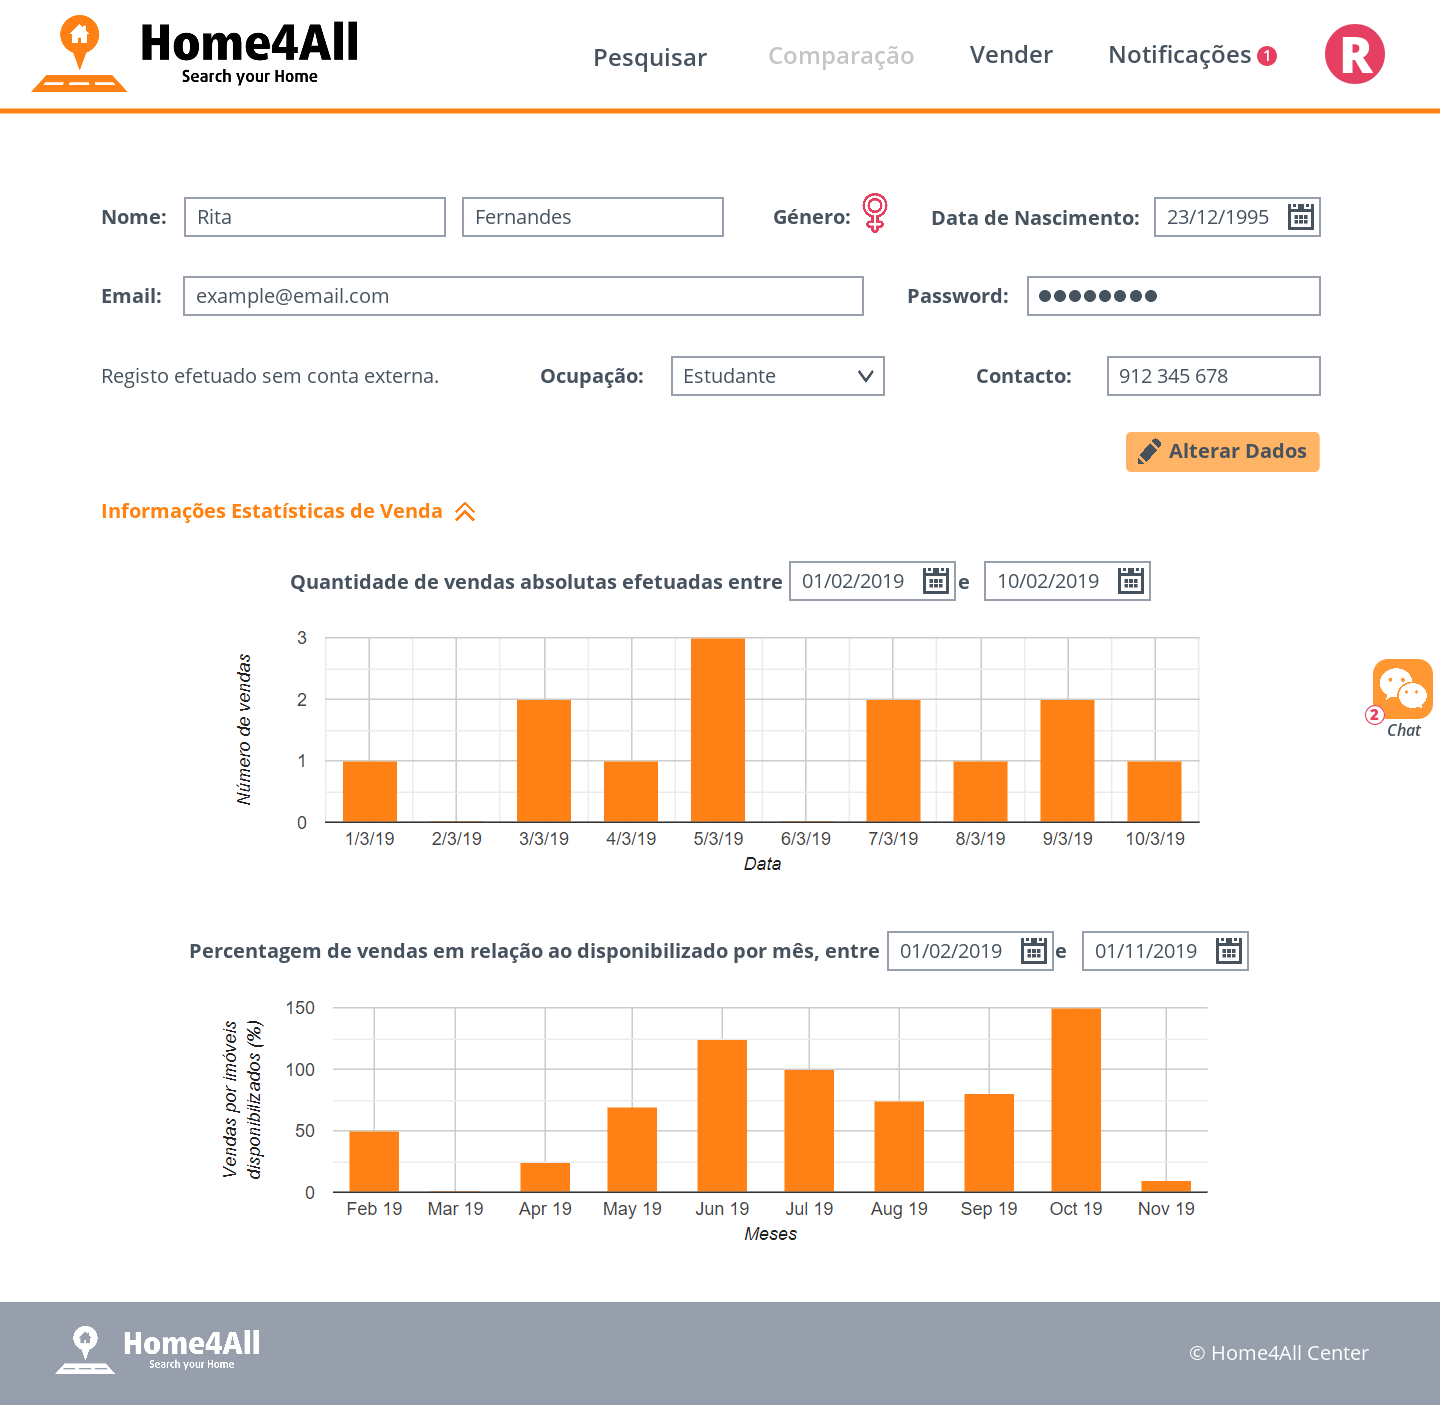
\includegraphics[width=0.9\textwidth]{./UI/PersonalInfo_WithStatistics.png}
    \caption{\textit{Mockup} da página com os dados pessoais do utilizador e estatísticas de venda.}
    \label{fig:personal_info_and_statistics}
\end{figure}

Neste caso, os princípios de usabilidade presentes são os seguintes:

\begin{itemize}
    \item \texttt{Learnability: Synthesizability} -- Quando se clica no botão para alteração dos dados, aparece uma mensagem de sucesso ou insucesso.
    
    \item \texttt{Learnability Familiarity} -- A forma de utilização do \textit{chat} privado é semelhante à de outros \textit{websites}, bem como o respetivo sistema de notificações.
    
    \item \texttt{Flexibility: Substitutivity} -- O contacto do utilizador pode ser escrito com ou sem o respetivo indicativo de país.
    
    \item \texttt{Robustness: Observability} --  Os botões para alterar dados e apresentar estatísticas de venda estão visíveis em ecrãs de tamanho médio e grande. Caso o tamanho do ecrã seja reduzido, o botão aparece imediatamente a seguir ao respetivo formulário, como de costume. As estatísticas de venda são consideradas informações adicionais, pelo que não lhes é atribuída demasiada importância. O \textit{chat} privado está sempre visível, numa posição fixa e independente do \textit{scroll}). As notificações no \textit{chat} funcionarão da mesma forma que as notificações de imóveis.
\end{itemize}


Dos \textit{design patterns} do \textit{website} \texttt{Designing Interfaces}, recorreu-se aos apresentados de seguida para esta página:

\begin{itemize}
    \item \texttt{Extras On Demand} -- Recorreu-se a este padrão para apresentar as informações estatísticas de venda. De facto, como estas são informações adicionais sobre o perfil, considerou-se que estes dados apenas deveriam ser apresentados mediante solicitação por parte do utilizador.
    
    \item \texttt{Input Prompt} -- A utilização de \textit{prompts} para indicar ao utilizador o que preencher, neste caso, deve-se ao facto dos dados já estarem inseridos por defeito. Nas situações anteriores, o utilizador deveria inserir os dados em campos vazios, pelo que se considerou suficiente que a informação sobre o que preencher apenas estivesse lá enquanto o utilizador não tivesse preenchido o respetivo campo.
    
    \item \texttt{Dropdown Chooser} -- A ocupação do utilizador pode ser selecionada de um \textit{dropdown}, que contém uma coleção variada de valores que podem ser escolhidos.
    
    \item \texttt{Edit-in-Place} -- Os campos referentes aos dados pessoais do utilizador são editáveis, servido os propósitos de consulta e edição.
\end{itemize}

Relativamente ao \textit{website} \texttt{Welie}, conseguiram-se utilizar os seguintes padrões de \textit{design}:

\begin{itemize}
    \item \texttt{Action Button} -- O botão ``Alterar Dados'' permite ao utilizador realizar uma ação relevante no contexto da página atual, pelo que é realçado com recurso a um ícone, bem como a cor e formato distintos (retângulo laranja com cantos arredondados). Para além disso, o \textit{label} do botão incluí o verbo da ação.
    
    \item \texttt{Date Selector} -- Caixa de texto editável, que também permite ao utilizador selecionar a data a partir de um calendário gráfico.
\end{itemize}

\subsubsection{Favoritos}

Em relação à página dos favoritos, criou-se um painel no qual se pode visualizar a hierarquia de diretorias existentes. Num segundo painel pode-se visualizar os imóveis armazenados na diretoria selecionada.

O \textit{mockup} da página dos favoritos é apresentado na figura \ref{fig:favorites}.

\begin{figure}[H]
    \centering
    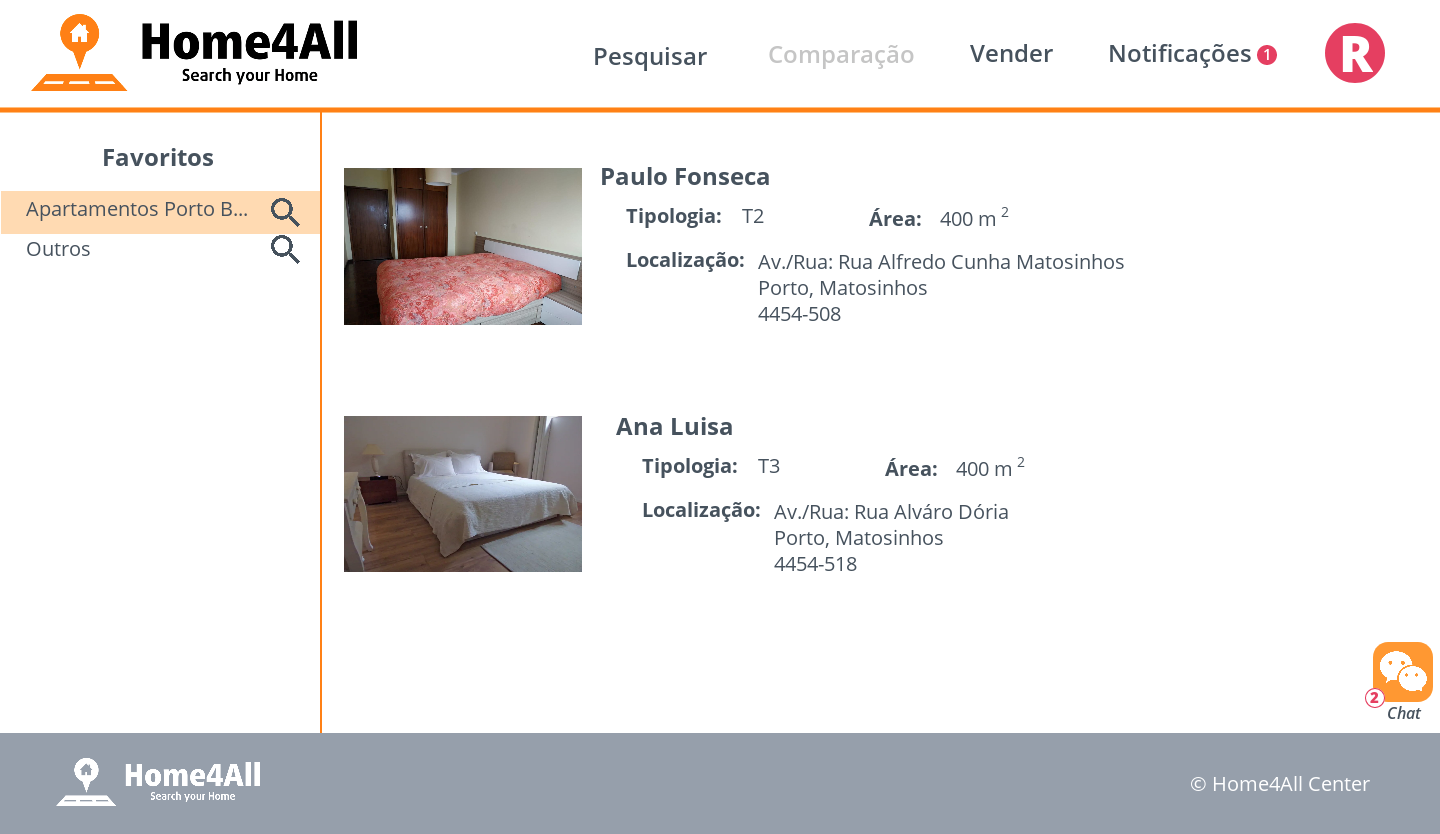
\includegraphics[width=0.9\textwidth]{./UI/Favorites.png}
    \caption{\textit{Mockup} da página dos favoritos.}
    \label{fig:favorites}
\end{figure}

Entre os vários \textit{design patterns} do \textit{website} \texttt{Designing Interfaces}, apenas foi utilizado o \texttt{Two-Panel Selector}. Recorreu-se a este padrão para desenhar dois painéis lado a lado, onde o primeiro mostra um conjunto de items (diretorias), que o utilizador pode selecionar conforme pretender, e o segundo mostra o conteúdo do item selecionado.

Quanto ao \textit{website} \texttt{Welie}, optou-se por utilizar o \textit{design pattern} \texttt{Paging}. Caso existam muitos imóveis associados à diretoria selecionada, será utilizado um sistema de \textit{paging} no segundo painel para facilitar a navegação por parte do utilizador.


\subsubsection{Configuração de Notificações}

Na página de configuração das notificações optou-se por recorrer ao mesmo sistema da página dos favoritos. Utilizaram-se dois painéis lado a lado, sendo que o primeiro apresenta todas as configurações existentes, enquanto que o segundo apresenta um formulário com as especificações dessa configuração, que podem ser alteradas.

Na figura \ref{fig:configurations} é apresentado o \textit{mockup} da página de configuração de notificações.

\begin{figure}[H]
    \centering
    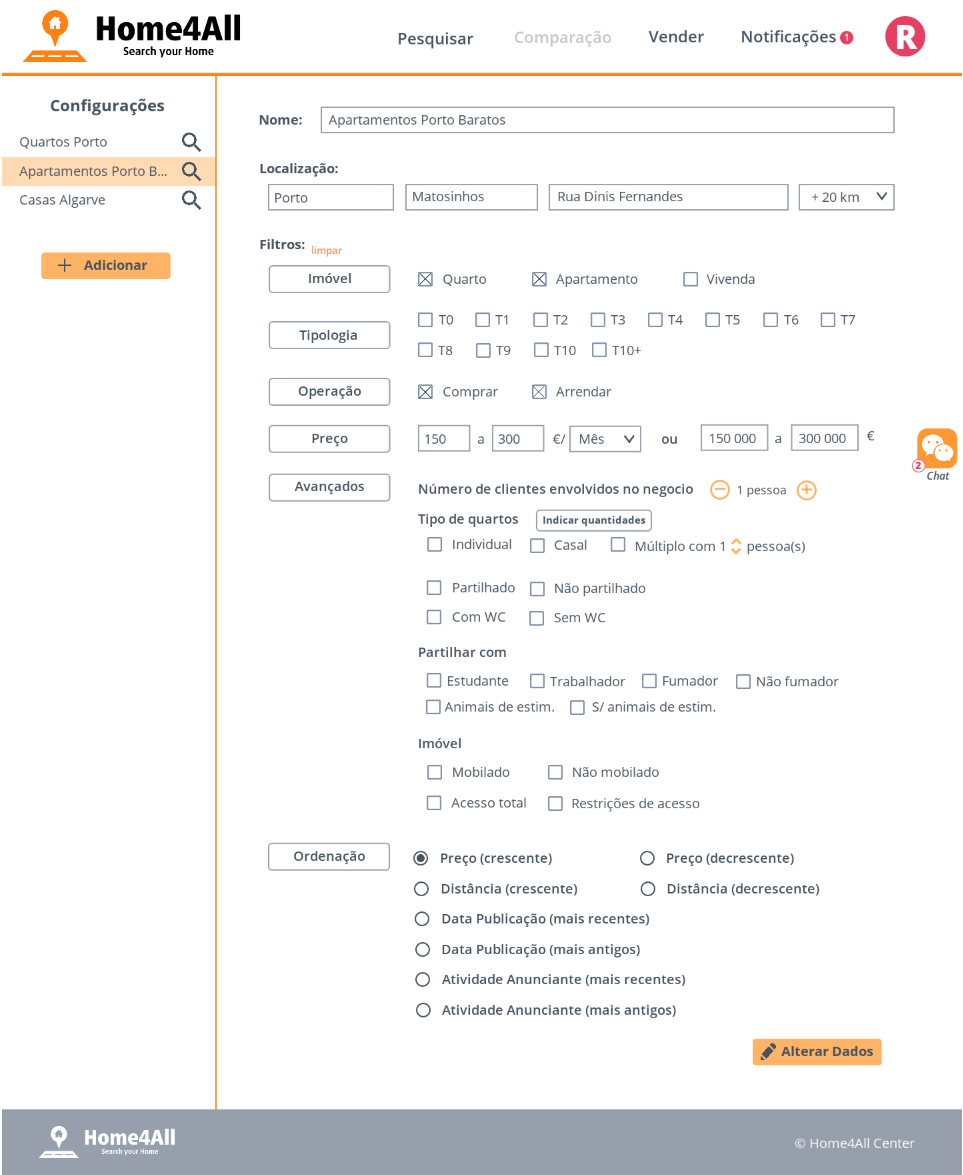
\includegraphics[width=0.85\textwidth]{./UI/Configurations.png}
    \caption{\textit{Mockup} da página com as configurações das notificações em vigor.}
    \label{fig:configurations}
\end{figure}

Em termos de princípios de usabilidade aplicados, destacam-se os seguintes:

\begin{itemize}
    \item \texttt{Learnability: Predictability} -- Quando o utilizador termina de inserir ou alterar o nome da configuração, o sistema indica erro se este já existir. O mesmo procedimento é seguido para a localização, quando esta não é encontrada, e para a distância ou o preço, caso sejam inválidos.
    
    \item \texttt{Learnability: Synthesizability} -- Após os dados de uma configuração serem alterados ou se adicionar uma nova configuração, será apresentada uma mensagem de sucesso ou insucesso.
    
    \item \texttt{Learnability: Consistency} -- São utilizados os mesmos campos e nomes (localização, filtros e ordenação) na página de pesquisa e nas configurações, o que facilita a previsão do tipo de resultados que serão obtidos.
    
    \item \texttt{Learnability: Familiarity} -- O preenchimento de formulários é comummente utilizado quando se pretende obter determinadas informações do utilizador.
    
    \item \texttt{Learnability: Generalizability/Consistency} -- A forma de apresentação e de consulta dos favoritos e das configurações é igual, o que facilita a aprendizagem do utilizador.
    
    \item \texttt{Flexibility: Substitutivity} -- A distância pode ser escrita, como um inteiro (que é interpretado como estando em quilómetros), ou pode ser selecionada de entre as opções disponíveis.
    
    \item \texttt{Robustness: Observability} -- O botão para alterar dados não está sempre visível, sendo necessário fazer \textit{scroll} para o visualizar. Contudo, desenhou-se a interface desta forma para garantir que o utilizador passa por todos os filtros possíveis, antes de alterar uma configuração.
\end{itemize}

Dos \textit{design patterns} do \textit{website} \texttt{Designing Interfaces}, recorreu-se aos apresentados de seguida para a página das configurações:

\begin{itemize}
    \item \texttt{Two-Panel Selector} -- Recorreu-se a este padrão para desenhar dois painéis lado a lado, onde o primeiro mostra um conjunto de items (configurações), que o utilizador pode selecionar conforme pretender, e o segundo mostra as especificações do item selecionado.
    
    \item \texttt{Dropdown Chooser} -- O distrito, a cidade e a distância podem ser selecionados de um \textit{dropdown}, que contém uma coleção variada de valores que podem ser escolhidos.
    
    \item \texttt{Edit-in-Place} -- Os campos referentes ao nome da configuração, localização procurada e filtros associados são editáveis, servido os propósitos de consulta e edição.
\end{itemize}

Relativamente ao \textit{website} \texttt{Welie}, conseguiram-se utilizar os seguintes padrões de \textit{design}:

\begin{itemize}
    \item \texttt{Action Button} -- O botão ``Alterar Dados'' permite ao utilizador realizar uma ação relevante no contexto da página atual, pelo que é realçado com recurso a um ícone, bem como a cor e formato distintos (retângulo laranja com cantos arredondados). Para além disso, o \textit{label} do botão inclui o verbo da ação.
    
    \item \texttt{Autocomplete} --  O campo da rua apresenta sugestões para completar o que está escrito, conforme o utilizador vai escrevendo.
    
    \item \texttt{Overview by Detail} -- No primeiro painel é apresentada uma vista geral sobre todas as configurações, identificadas pelo respetivo nome. No segundo, é indicada a especificação da configuração selecionada. Desta forma, o utilizador consegue inspecionar as várias configurações, sem ter de mudar de página constantemente para voltar à vista geral.
    
    \item \texttt{Form} -- Utilizou-se um formulário para solicitar ao utilizador a introdução das especificações de cada configuração de notificação (nome, localização e filtros).
\end{itemize}


\subsubsection{Anunciar Novo Imóvel}

Relativamente à página de anúncio de um novo imóvel, optou-se por utilizar um formulário que o anunciante pudesse preencher com todas as informações necessárias sobre o imóvel. O respetivo \textit{mockup} é apresentado na figura \ref{fig:announce}.
 
\begin{figure}[H]
    \centering
    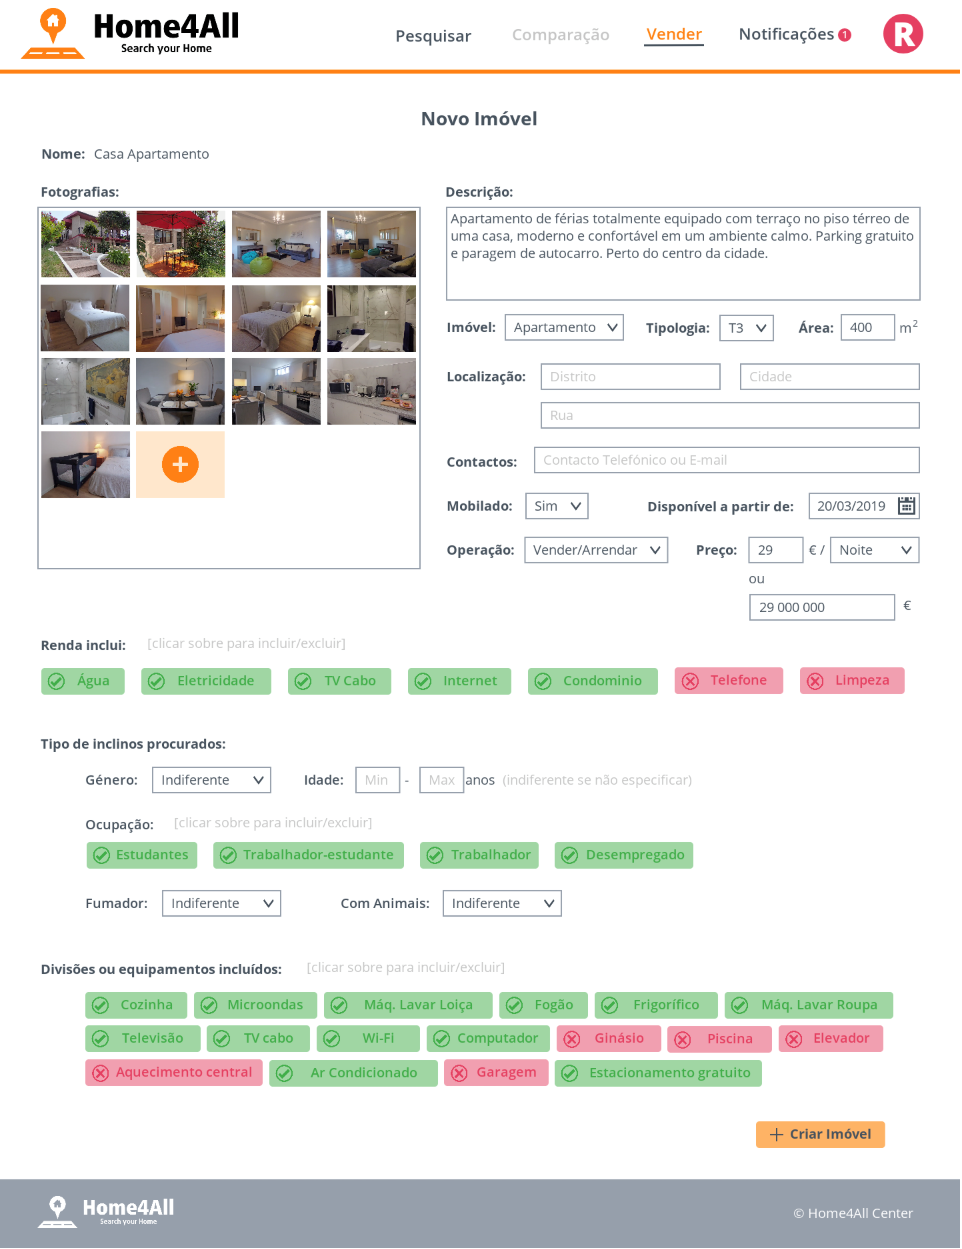
\includegraphics[width=0.9\textwidth]{./UI/Vender.png}
    \caption{\textit{Mockup} da página onde um anunciante introduz os dados de um novo imóvel.}
    \label{fig:announce}
\end{figure}

Nesta página conseguiu-se aplicar os princípios de usabilidade apresentados de seguida:

\begin{itemize}
    \item \texttt{Learnability: Predictability} -- Quando o utilizador termina de inserir o nome do imóvel, o sistema indica erro se este já existir. O mesmo procedimento é seguido para a localização, quando esta não é encontrada, e para a área, contacto, preço ou idade, caso sejam introduzidos valores inválidos.
    
    \item \texttt{Learnability: Synthesizability} -- Após o utilizador adicionar o imóvel, o sistema devolverá uma mensagem de sucesso ou insucesso.
    
    \item \texttt{Learnability: Familiarity} -- O preenchimento de formulários é comummente utilizado quando se pretende obter determinadas informações do utilizador.
    
    \item \texttt{Learnability: Generalizability/Consistency} -- A ordem de apresentação dos campos no formulário é a mesma que quando se consulta a página de um imóvel, o que permite uma maior familiarização com as informações solicitadas, por parte do utilizador.
    
    \item \texttt{Flexibility: Substitutivity} -- A distância pode ser escrita, como um inteiro (que é interpretado como estando em quilómetros), ou pode ser selecionada de entre as opções disponíveis.
    
    \item \texttt{Robustness: Observability} -- O botão para criar imóvel não está sempre visível, sendo necessário fazer \textit{scroll} para o visualizar. Contudo, desenhou-se a interface desta forma para garantir que o utilizador passa por todos os campos que é necessário indicar antes de adicionar o imóvel. De facto, caso o utilizador não tenha preenchido algum campo obrigatório, será avisado ao tentar criar o imóvel. No entanto, existem alguns campos que já têm um valor por defeito, pretendendo-se que o utilizador os analise antes de submeter o formulário.
\end{itemize}

Entre os padrões de \textit{design} do \textit{website} \texttt{Designing Interfaces}, utilizaram-se os seguintes:

\begin{itemize}
    \item \texttt{Fill-in-the-Blanks} -- Utilizou-se este padrão para se indicar um intervalo de preços e a quantidade de pessoas no quarto múltiplo.
    
    \item \texttt{Dropdown Chooser} -- O distrito e a cidade podem ser selecionados de um \textit{dropdown}, que contém uma coleção variada de valores que podem ser escolhidos.
\end{itemize}

Quanto ao \textit{website} \texttt{Welie}, utilizaram-se os seguintes \textit{design patterns}:

\begin{itemize}
    \item \texttt{Action Button} -- O botão ``Criar Imóvel'' permite ao utilizador realizar a ação principal no contexto da página atual, pelo que é realçado com recurso a uma cor e um formato distintos (retângulo laranja com cantos arredondados). Para além disso, o \textit{label} do botão inclui o verbo da ação.

    \item \texttt{Autocomplete} -- O campo da rua apresenta sugestões para completar o que está escrito, conforme o utilizador vai escrevendo.
    
    \item \texttt{Thumbnail} -- Imagens dos imóveis mais pequenas são apresentadas para permitir ao anunciante verificar de forma direta quais as fotografias cujo \textit{upload} já efetuou.
    
    \item \texttt{Date Selector} -- Caixa de texto editável, que também permite ao utilizador selecionar a data a partir de um calendário gráfico.
    
    \item \texttt{Form} -- Utilizou-se um formulário para solicitar ao utilizador a introdução das informações específicas sobre o imóvel a anunciar.
\end{itemize}


\subsection{Técnicas de Avaliação da Usabilidade}

A usabilidade foi um dos aspetos fundamentais que acompanharam o
desenvolvimento do projeto desde do início até ao fim. O objetivo passou por
criar uma aplicação que fosse intuitiva e fácil de utilizar. No entanto, a
opinião da equipa de desenvolvimento é claramente distorcida e, por isso, foi
importante recorrer a métodos credíveis para que a avaliação pudesse ser
confiável.

Desta forma, a estratégia adotada passava por realizar dois momentos de
avaliação, um utilizando o \textit{mockup} inicial da interface e outro quando a
interface estiver implementada a ponto de poder ser testada. Por um lado, numa
primeira fase consegue-se recolher \textit{feedback} de forma a ajustar o
desenvolvimento em si. Por outro lado, a segunda avaliação permite tirar
conclusões à cerca do trabalho desenvolvido e realizar pequenos ajustes se
assim for necessário.

Além disso, cada momento de avaliação vai incorporar dois tipos de testes
diferentes. Destes, um será um teste de usabilidade onde vários indivíduos
serão monitorizados, enquanto executam várias tarefas previamente escolhidas. No
fim, cada participante irá responder ao questionário \textit{System Usability Scale} (SUS). Deste teste
espera-se recolher \textit{feedback} relacionado com a eficácia, eficiência e
satisfação na utilização da ferramenta. O segundo teste é o \textit{cognitive
walkthrough} e já utiliza um método analítico. Este, realizado pelos elementos
da equipa de desenvolvimento, permitirá identificar possíveis problemas e a
respetiva severidade.

As secções que se seguem descrevem em pormenor o processo utilizado para
avaliar a usabilidade do projeto, assim como os resultados obtidos nesses
mesmos testes.

\subsubsection{Método empírico - Teste de usabilidade}
\label{sec:orgcf0b6f9}
\paragraph{Objetivos}
\label{sec:org95e7a36}
O primeiro passo no método empírico está relacionado com a definição dos
objetivos que se pretende atingir ao realizar o teste em si. Desta forma,
existe três grandes componentes que devem ser abordadas, nomeadamente a
\textbf{eficácia}:

\begin{itemize}
\item registando o rácio de sucesso/insucesso das diferentes tarefas propostas;
\item quantificando os problemas sentidos pelos utilizadores;
\end{itemize}

%a \textbf{eficiência}:

%\begin{itemize}
%\item registando o tempo necessário para executar determinadas tarefas;
%\item tempo gasto a consultar documentação/outras ajudas;
%\item tempo gasto a resolver erros;
%\end{itemize}

e a \textbf{satisfação}:

\begin{itemize}
\item utilizando questionários.
\end{itemize}

Desta forma, espera-se recolher dados suficientes para tirar conclusões à
cerca da usabilidade da interface implementada.

\paragraph{Tarefas a realizar}
\label{sec:orgea1fb37}
Um aspeto importante nos testes de usabilidade é o estabelecimento das
tarefas que vão ser realizadas. Achou-se que o melhor seria utilizar duas
tarefas diferentes. Por um lado, se fossem realizadas mais, o tempo
necessário para a realização do teste aumentaria e os utilizadores não iriam
produzir resultados tão úteis devido ao possível cansaço sentido. Por outro
lado, apenas um teste levaria a resultados que iriam estar completamente
dependentes do teste em si, o que não permitia ter uma visão generalizada da
usabilidade do sistema.

Assim sendo, os cenários escolhidos são:

\begin{itemize}
\item adicionar um quarto duplo para arrendar. Características: mobilado, casa
de banho partilhada, disponível a partir de  de 10/08/2019, 300€ por mês.
Renda incluí: água, eletricidade, Internet. Tipo de inquilinos procurados:
género masculino, estudante, não fumador, sem animais de estimação.
Divisões/equipamentos disponíveis: cozinha, micro-ondas, fogão,
frigorífico, televisão, \textit{wi-fi}, elevador, estacionamento gratuito.
Arrendatários atuais: 0 animais de estimação, 3 estudantes do género
masculino e nenhum é fumador.
\item consulte o imóvel que acabou de registar.
\item alterar informações pessoais.
\item procurar um quarto em Carnaxide para arrendar com valor máximo de 400€.
\item alterar informações pessoais.
\end{itemize}

De facto, dado que as tarefas são de natureza e contexto diferente,
espera-se obter uma ideia mais alargada da usabilidade da ferramenta.

\paragraph{Execução do estudo}
\label{sec:orgaff5f0e}
Após realizada toda a preparação anteriormente especificada, a execução do
teste propriamente dita pode ser realizada. Na prática, é dado ao utilizador
um contexto detalhado do processo que vai ser realizado. De seguida, os
participantes realizam o teste, durante o qual, o observador vai recolhendo
as devidas notas. Por fim, o estudo termina com a realização dos
questionários definidos na fase de preparação.

De realçar, que será pedido ao participante que vá explicando o seu raciocínio
enquanto realiza as tarefas, assim como expresse a sua opinião ao longo do
processo.

De facto, com esta tipologia de teste espera-se recolher os dados
necessários para retirar conclusões significativas.

\paragraph{Processamento dos dados}
\label{sec:org2aedb1d}

\begin{itemize}
    \item Contar as tarefas realizadas com sucesso/insucesso
    \item Recolher opinião
    \item Estatísticas do questionário
\end{itemize}

\subsubsection{Método analítico - Inspeção por peritos}
\label{sec:org7ae4da1}
\paragraph{Objetivos}
\label{sec:org8305494}
O método analítico é também incorporado no capítulo da avaliação da
usabilidade, mas este tem um objetivo possivelmente diferente. Efetivamente,
o método analítico permite prever potenciais problemas de usabilidade e não
tanto avaliar a usabilidade em si. Desta forma, consegue-se corrigir os
problemas de modo a ter uma avaliação mais positiva da usabilidade.

No caso específico deste projeto o teste escolhido foi o \textit{cognitive
walkthrough}, que pretende dar resposta à pergunta: até que ponto o sistema
vai guiar um utilizador não treinado na execução de uma dada tarefa?

\paragraph{Descrição dos utilizadores}
\label{sec:orgf382e34}

Uma componente importante neste tipo de testes passa por ter em conta o tipo
utilizador que vai utilizar a ferramenta. Desta forma, a realização dos testes vai ser feita de modo a simular o raciocínio tido por cada uma das \textit{personas} identificadas em \ref{sec:personas}. Desta maneira espera-se obter resultados
mais fidedignos.

\paragraph{Tarefas a realizar}
\label{sec:org9167ec4}
As tarefas a avaliar neste teste são as que se encontram descritas na secção
\ref{sec:orgea1fb37} e, adicionalmente,
uma que simule o arrendamento de um quarto.

No entanto, importa realçar que a equipa de desenvolvimento encontra-se
responsável por realizar este teste em qualquer momento que achar oportuno,
sendo que nesses casos a avaliação não será adicionada neste documento.

\paragraph{Execução do estudo}
\label{sec:org18926e1}
A execução deste teste é bastante simples e consiste em responder a quatro
questões:

\begin{enumerate}
\item A ação correta é suficientemente evidente para o utilizador? [Sim / Não]
\item O controlo para executar a ação está visível? [Sim / Não]
\item Irá o utilizador associar a ação correta ao controlo? [Sim / Não]
\item Irá o utilizador interpretar de forma correta a resposta do sistema à
ação escolhida? [Sim / Não]
\end{enumerate}

De facto, para cada pergunta, caso a resposta seja negativa, então deve ser
especificada a severidade do problema encontrado da seguinte forma:

\begin{itemize}
\item \textbf{Tipo 1}: o problema pode causar confusão ou demora na execução da tarefa.
\item \textbf{Tipo 2}: o problema pode impedir que o utilizador consiga executar a tarefa
sem ajuda.
\item \textbf{Tipo 3}: o problema impede a execução da tarefa.
\end{itemize}

Adicionalmente, sempre que possível deve ser acrescentada uma descrição do
problema encontrado assim como uma sugestão para este.

Assim sendo, espera-se conseguir prever alguns dos problemas que surjam ao
longo do desenvolvimento do projeto e assim obter uma melhor avaliação de
usabilidade à partida.

\paragraph{Processamento dos dados}
\label{sec:org2d14279}

De seguida, apresentam-se então os resultados dos testes de usabilidade executados com base nos \textit{mockups} desenvolvidos bem como as taxas de completude das tarefas constituintes do teste respetivamente.

\begin{table}[H]
\centering
\caption{Resultados do questionário SUS para os \textit{mockups} e respetivos \textit{scores}.}
\begin{tabular}{ccccccccccc}
\hline
\rowcolor[HTML]{EFEFEF} 
\textbf{1} & \textbf{2} & \textbf{3} & \textbf{4} & \textbf{5} & \textbf{6} & \textbf{7} & \textbf{8} & \textbf{9} & \textbf{10} & \textbf{TOTAL} \\ \hline
3          & 2          & 4          & 2          & 4          & 2          & 4          & 2          & 3          & 1           & 72.5           \\
4          & 2          & 3          & 1          & 5          & 2          & 4          & 2          & 3          & 2           & 75             \\
3          & 3          & 3          & 1          & 3          & 2          & 3          & 2          & 3          & 2           & 62.5           \\
3          & 2          & 4          & 1          & 5          & 1          & 4          & 1          & 4          & 1           & 85             \\ \hline
\end{tabular}
\end{table}


\begin{table}[H]
\centering
\caption{Resultados da completude das tarefas realizadas durante os testes e respetivos \textit{scores}.}
\begin{tabular}{ccccc}
\hline
\rowcolor[HTML]{EFEFEF} 
\textbf{1} & \textbf{2} & \textbf{3} & \textbf{4} & \textbf{TOTAL} \\ \hline
0.5        & 1          & 1          & 1          & 88\%           \\
1          & 1          & 1          & 1          & 100\%           \\
1          & 1          & 1          & 0,5        & 88\%           \\
1          & 1          & 1          & 1          & 100\%           \\ \hline
\end{tabular}
\end{table}

Em suma, apesar dos resultados não revelarem resultados 100\% positivos, ainda assim revelaram-se bastante positivos.